\documentclass[12pt, a4paper, oneside]{article}
\usepackage[default]{opensans}
\usepackage{geometry}
\usepackage{lipsum}
\usepackage[spanish]{babel}
\usepackage{graphicx}
\usepackage{pdfpages}
\usepackage{xcolor}
\usepackage{titlesec}
\usepackage{blindtext}


\usepackage{mwe}
\usepackage[hidelinks]{hyperref}

\usepackage{bookmark}

\usepackage{amsmath}
\usepackage{array}

\usepackage{amsmath}
\usepackage[mathrm=sym]{unicode-math}
\setmathfont{Fira Math}

\newcommand\invisiblesection[1]{%
  \refstepcounter{section}%
  \addcontentsline{toc}{section}{\protect\numberline{\thesection}#1}%
  \sectionmark{#1}}



\begin{document}


\includepdf[pages=1,scale=0.90]{MAIN_COVER_PAGE.pdf}
\pdfbookmark[section]{\contentsname}{toc}
\tableofcontents
\newpage

\invisiblesection{Abstract}
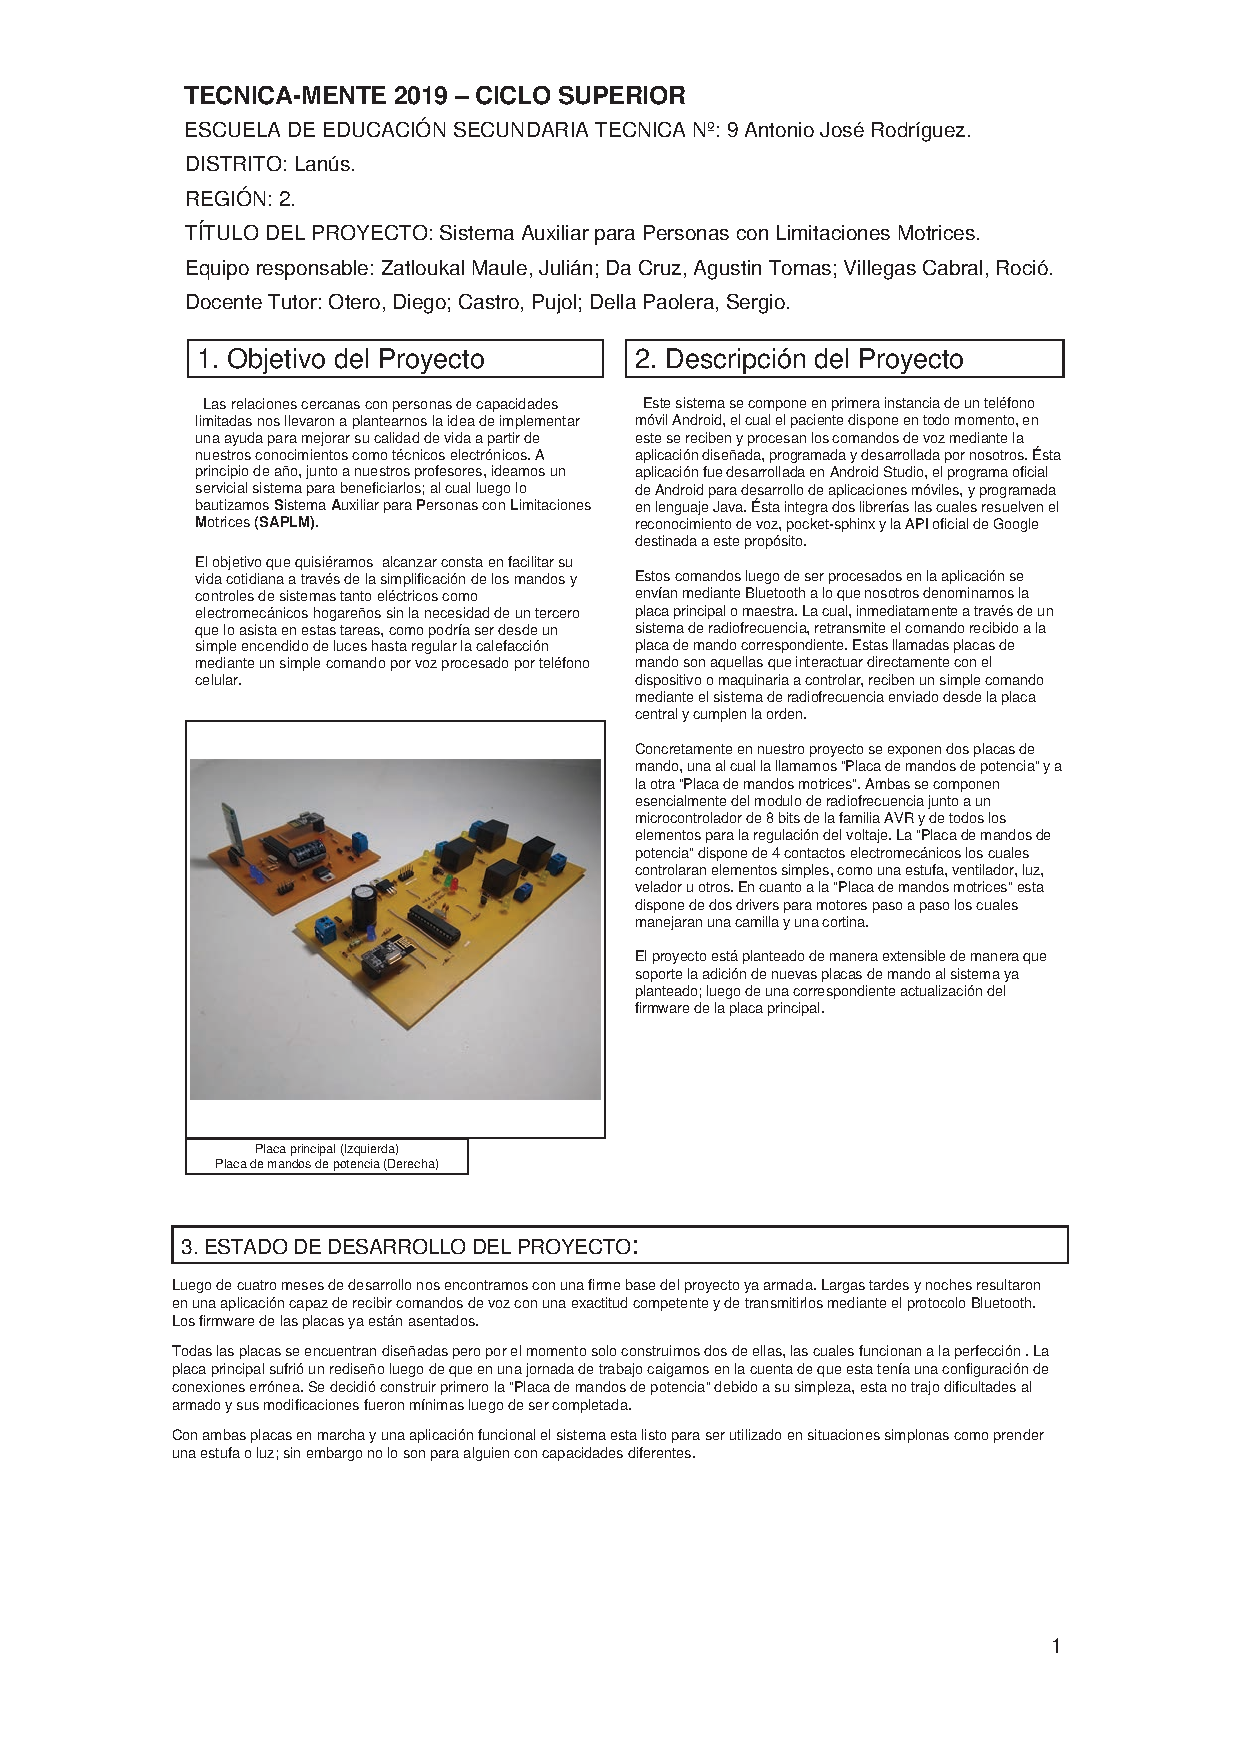
\includepdf[scale=1.00, pagecommand={}]{ABSTRACT.pdf}

\invisiblesection{Diagrama en bloques}
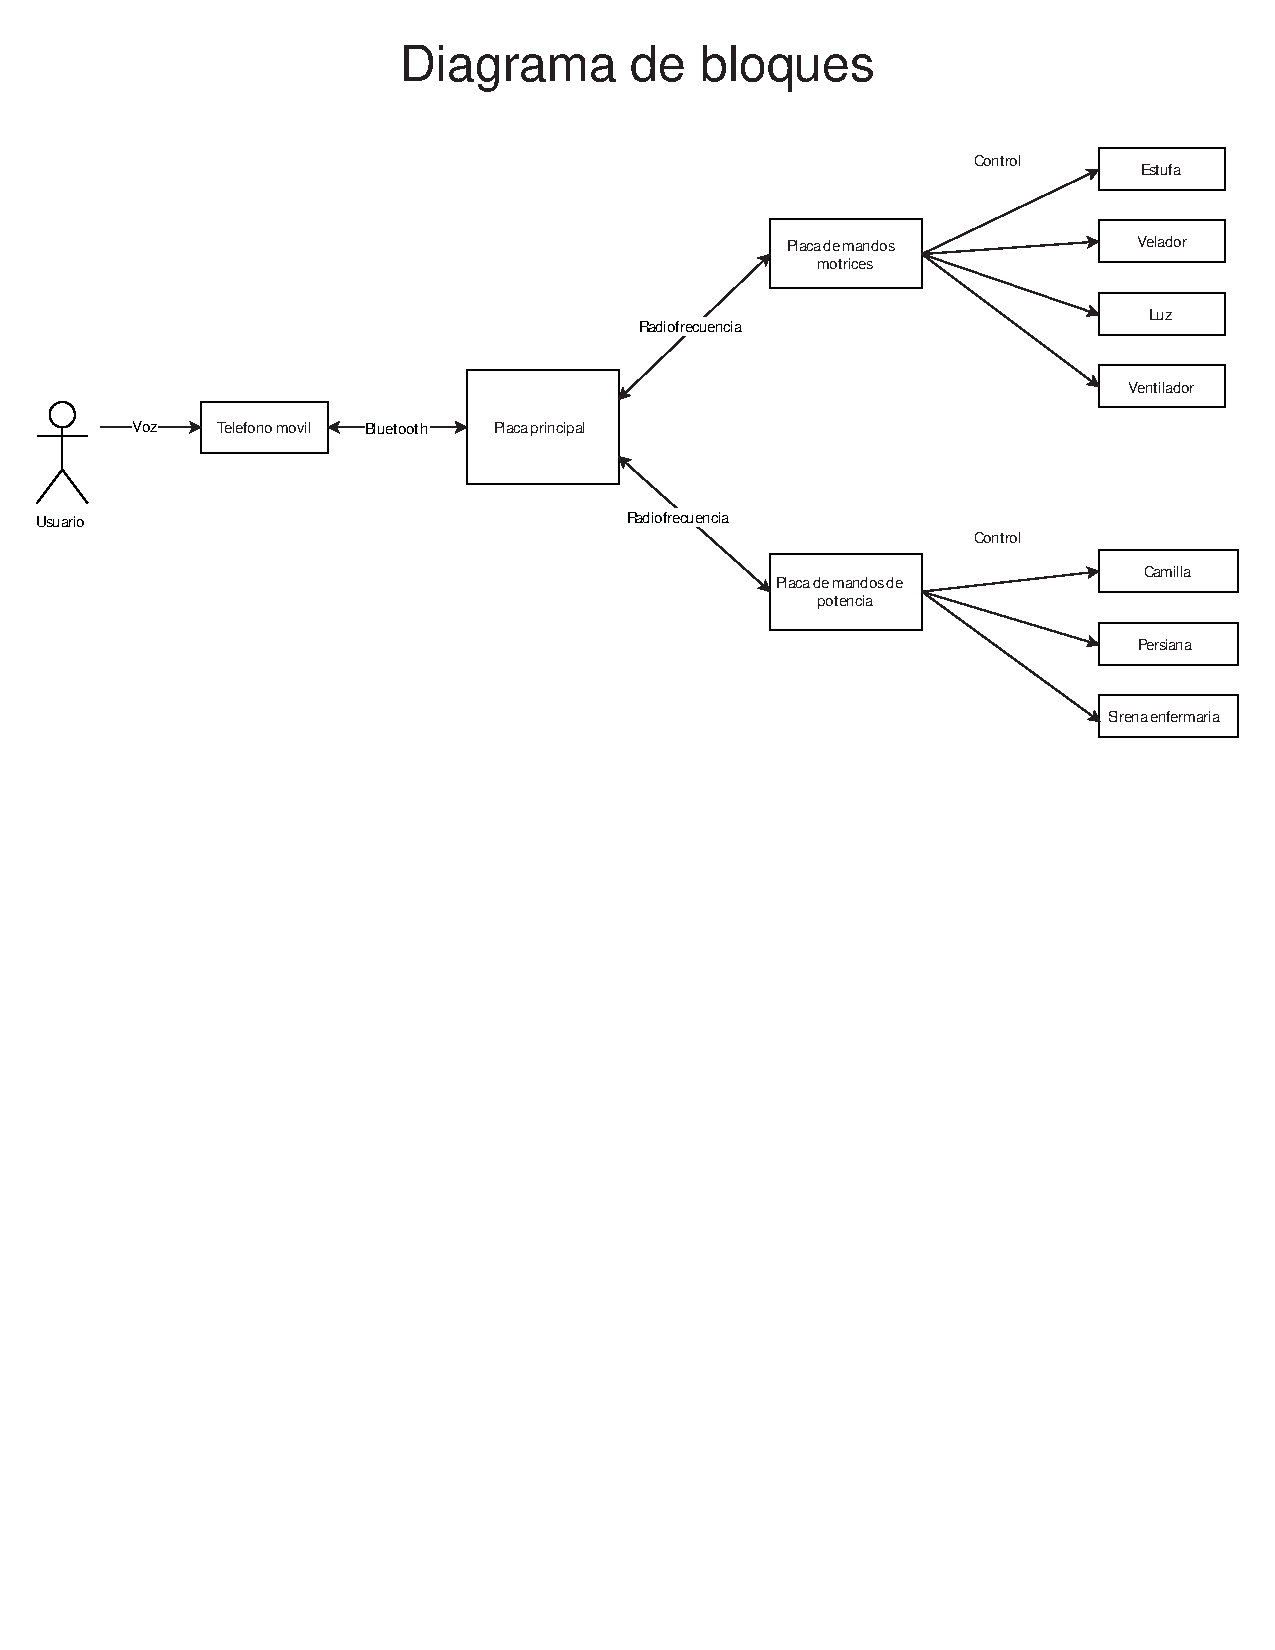
\includepdf[scale=1.00, pagecommand={}]{DIAGRAMA_BLOQUES.pdf}

\invisiblesection{Diagrama de flujo para encender estufa}
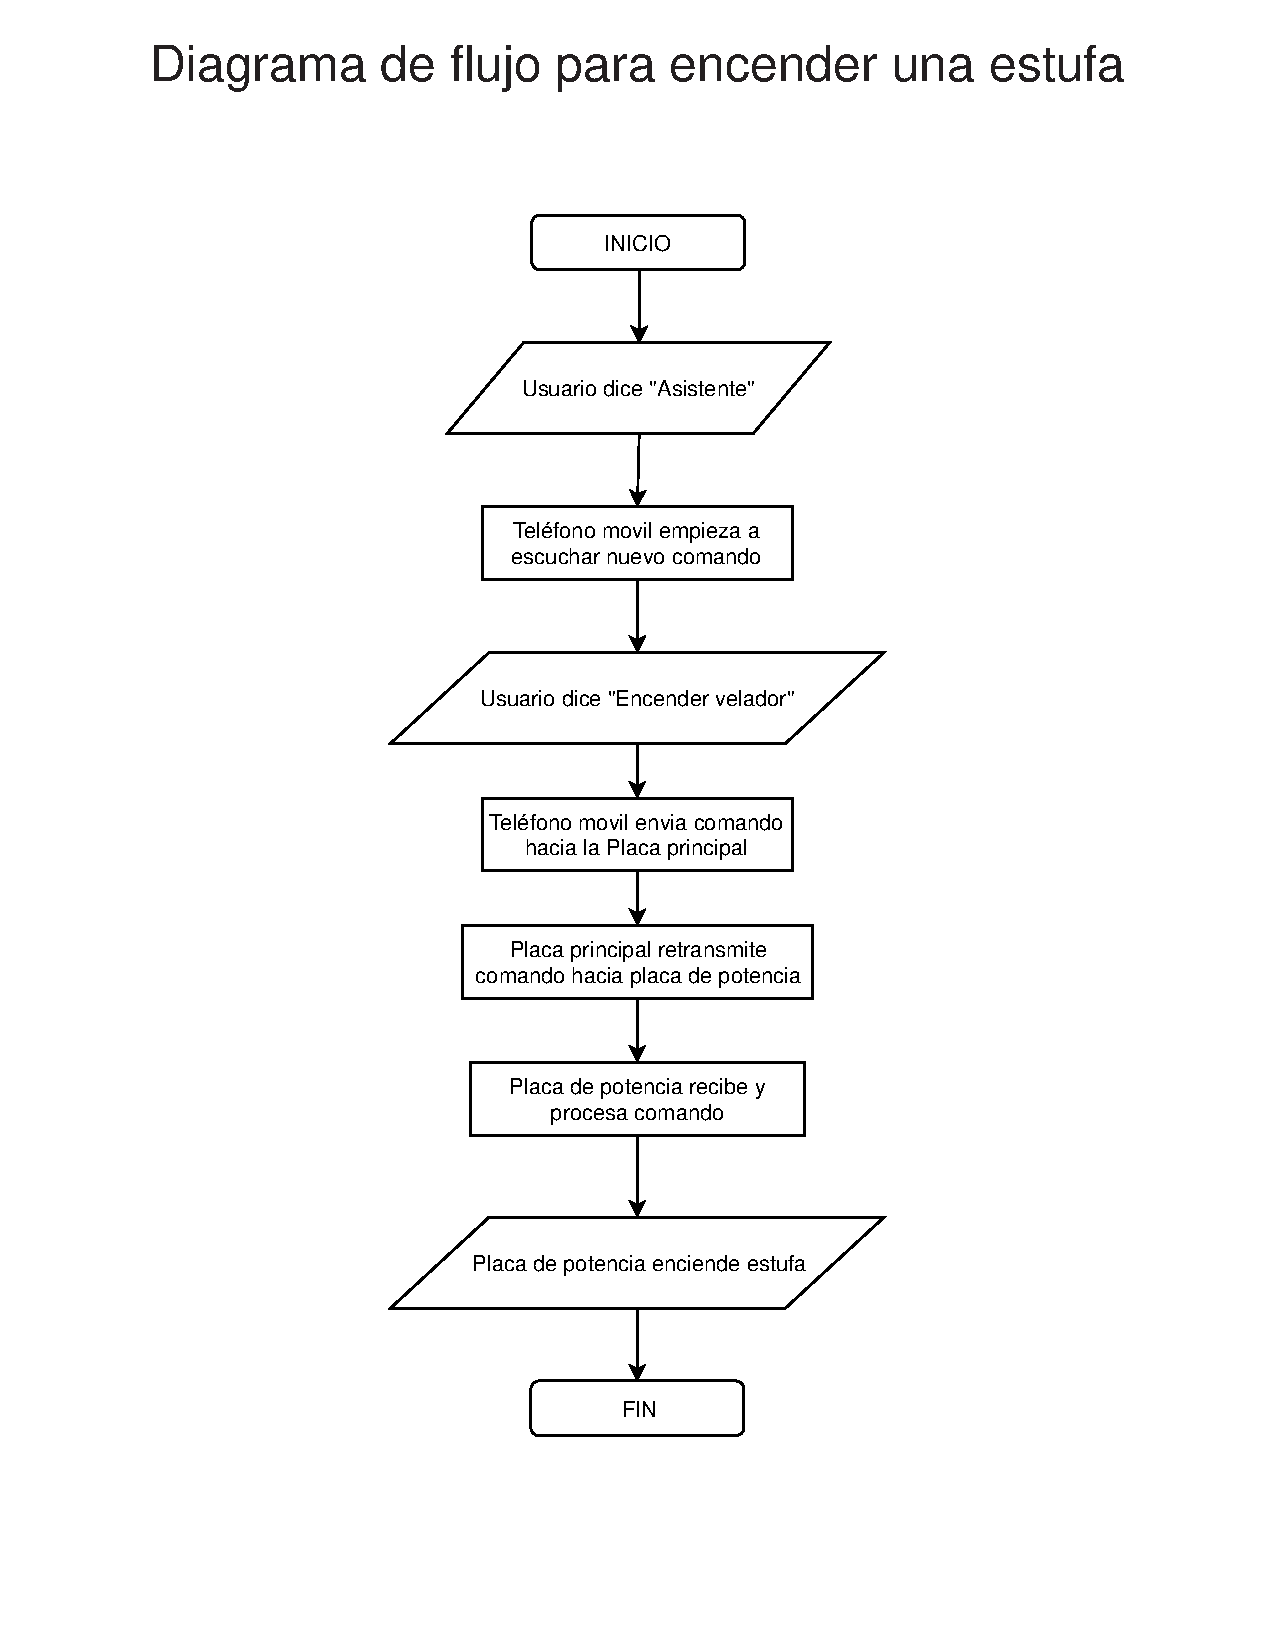
\includepdf[scale=1.00, pagecommand={}]{DIAGRAMA_FLUJO_MAIN.pdf}

\invisiblesection{Comandos de voz disponibles}
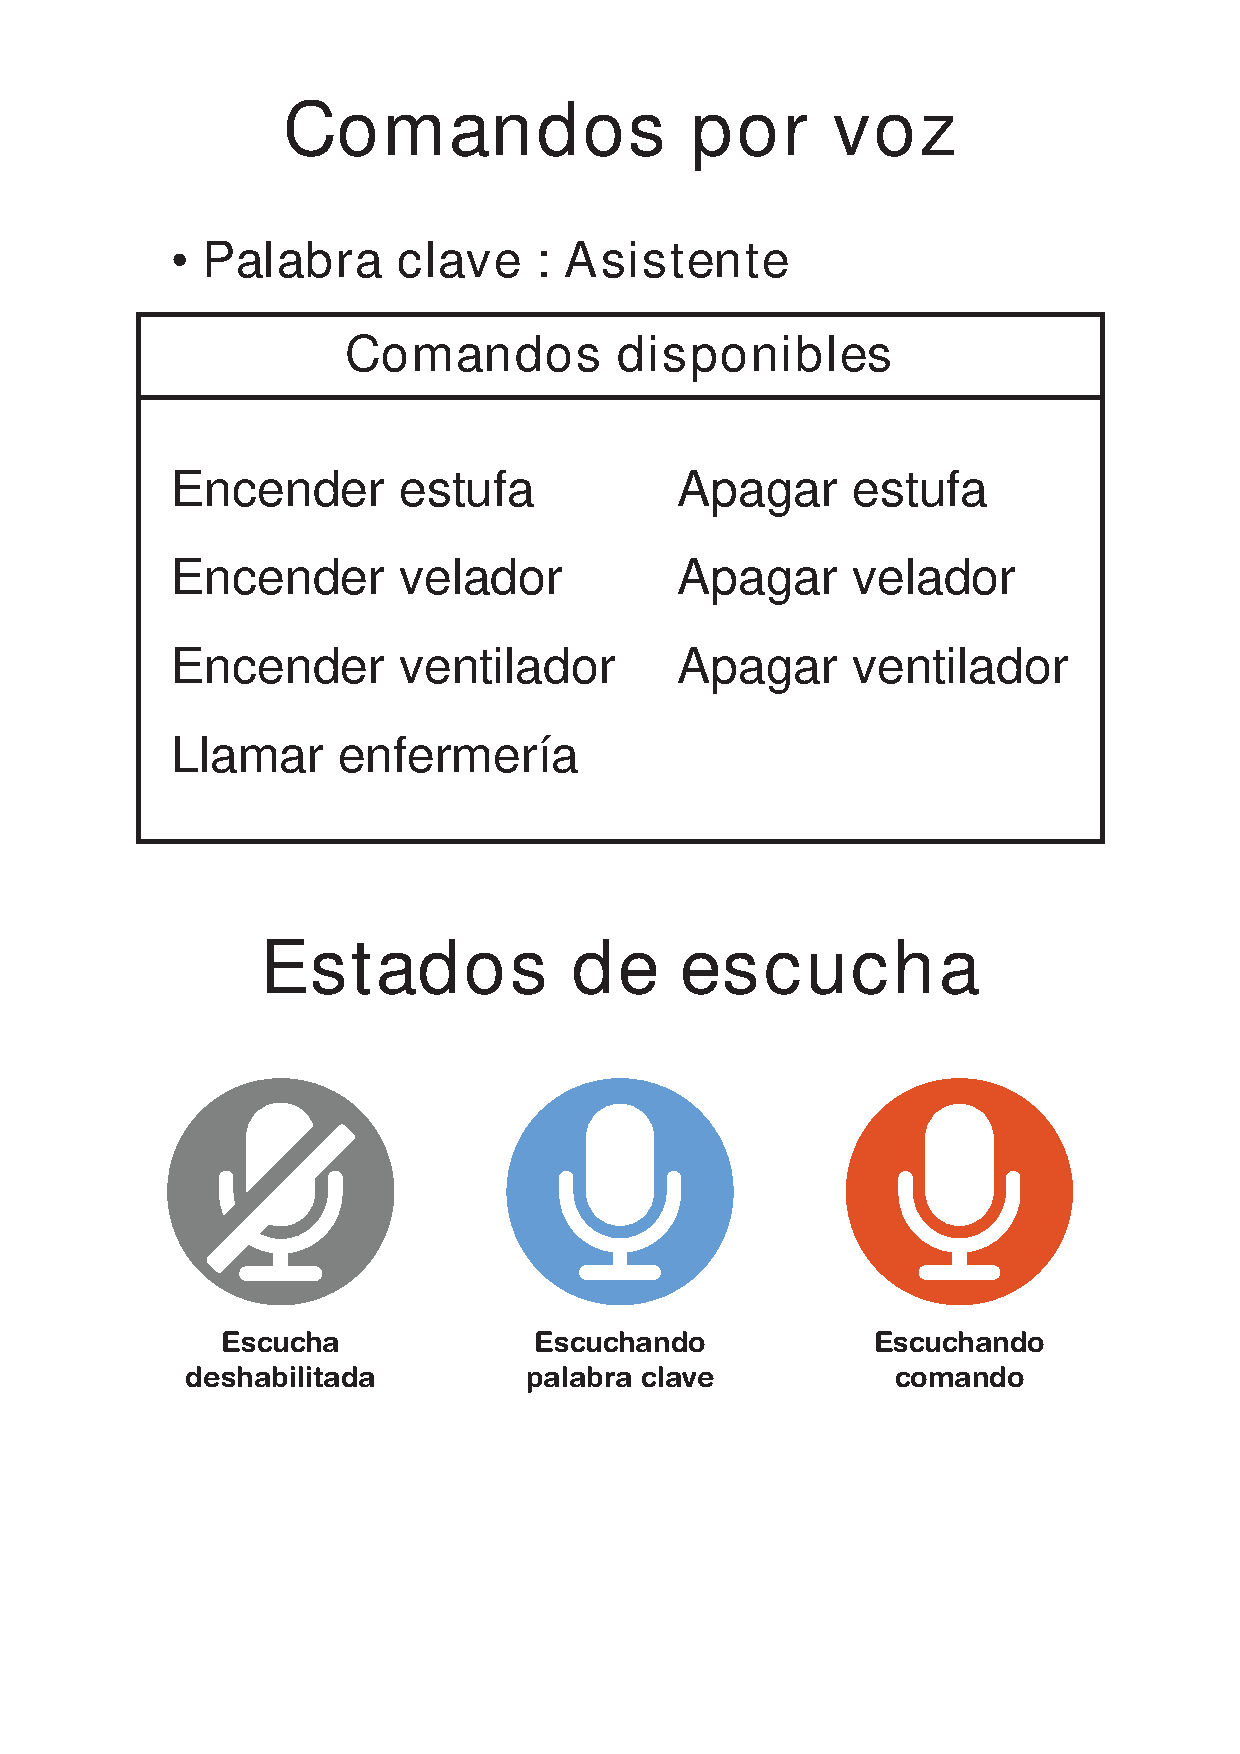
\includepdf[scale=1.00, pagecommand={}]{VOICE_COMMANDS.pdf}

\invisiblesection{Diagrama de flujo}
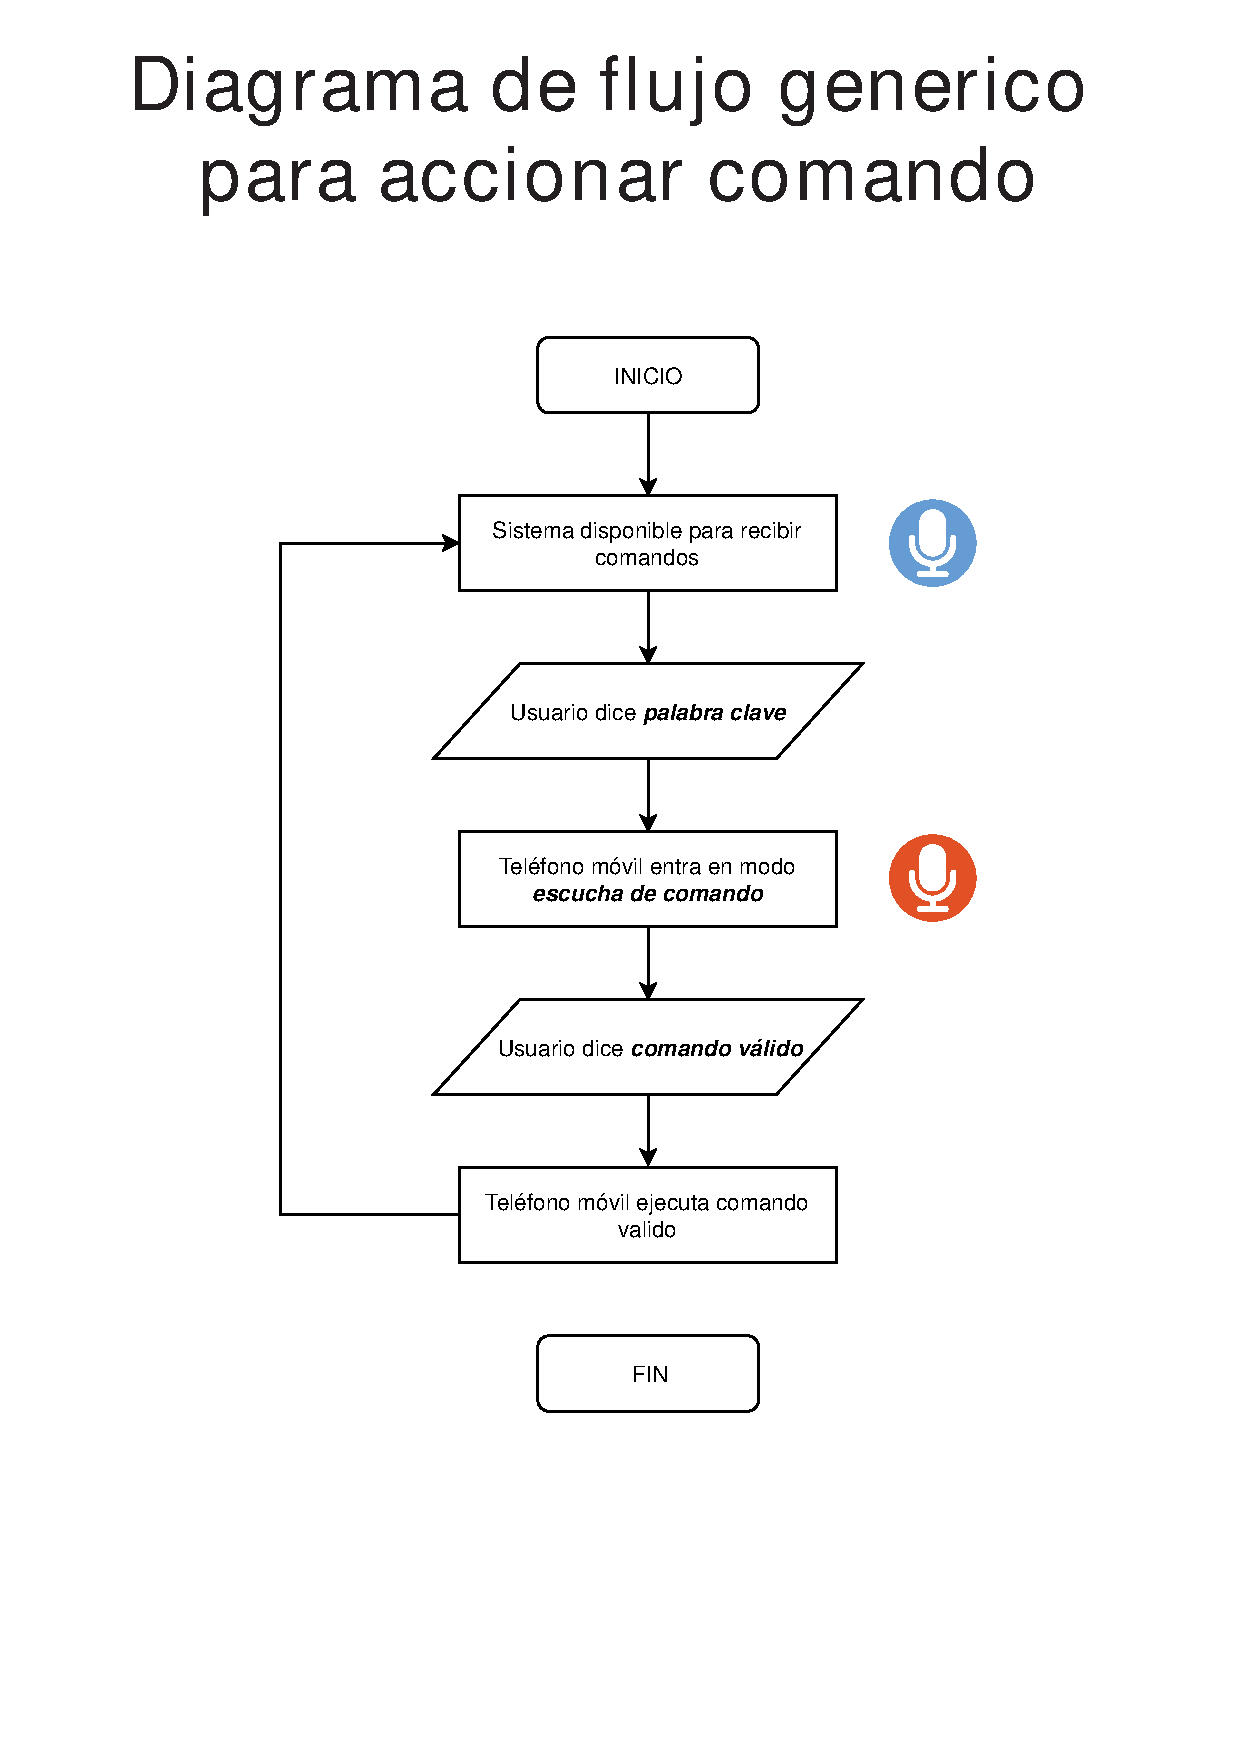
\includepdf[scale=1.00, pagecommand={}]{DIAGRAMA_FLUJO_SECOND.pdf}

\invisiblesection{Imagenes de la aplicación}
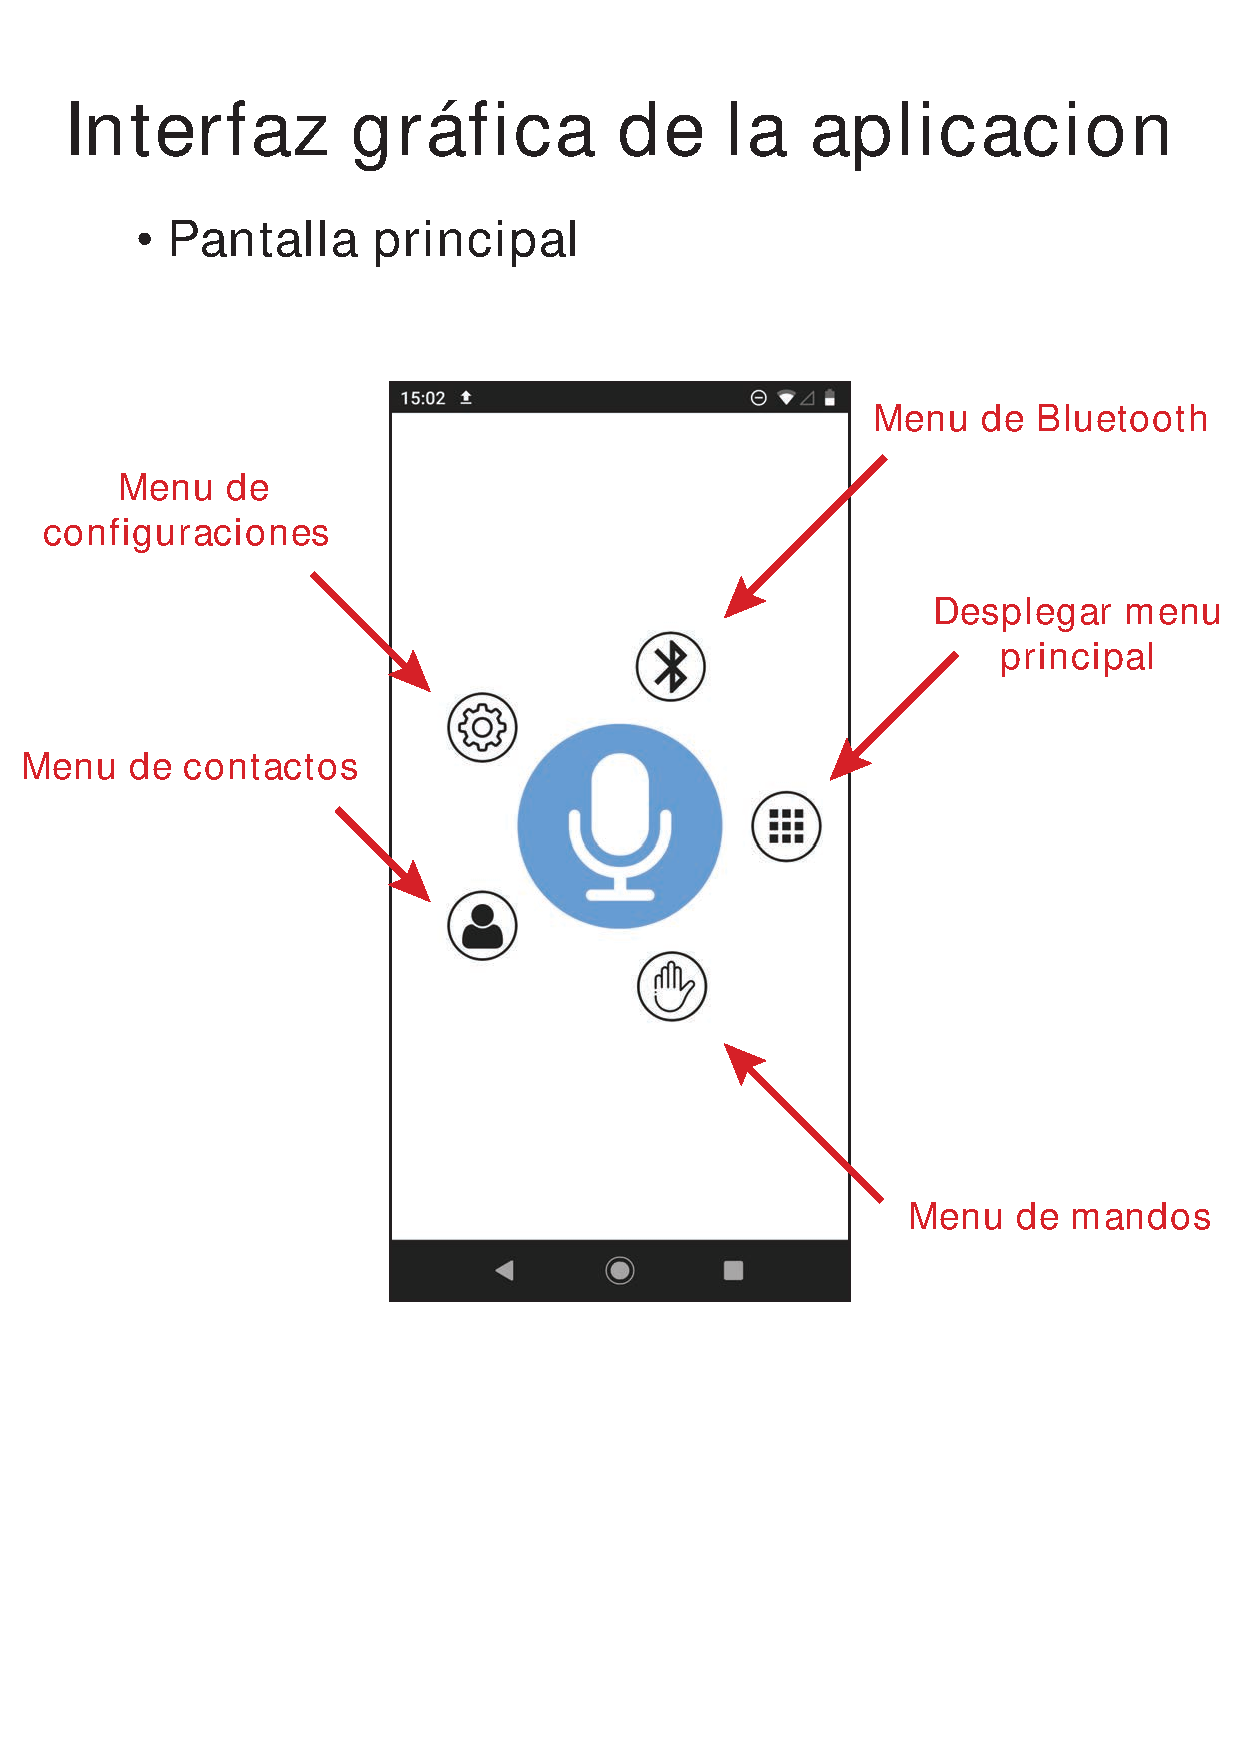
\includepdf[pages={1-},scale=1.00, pagecommand={}]{APP_IMAGES.pdf}

\invisiblesection{Carpeta de campo}
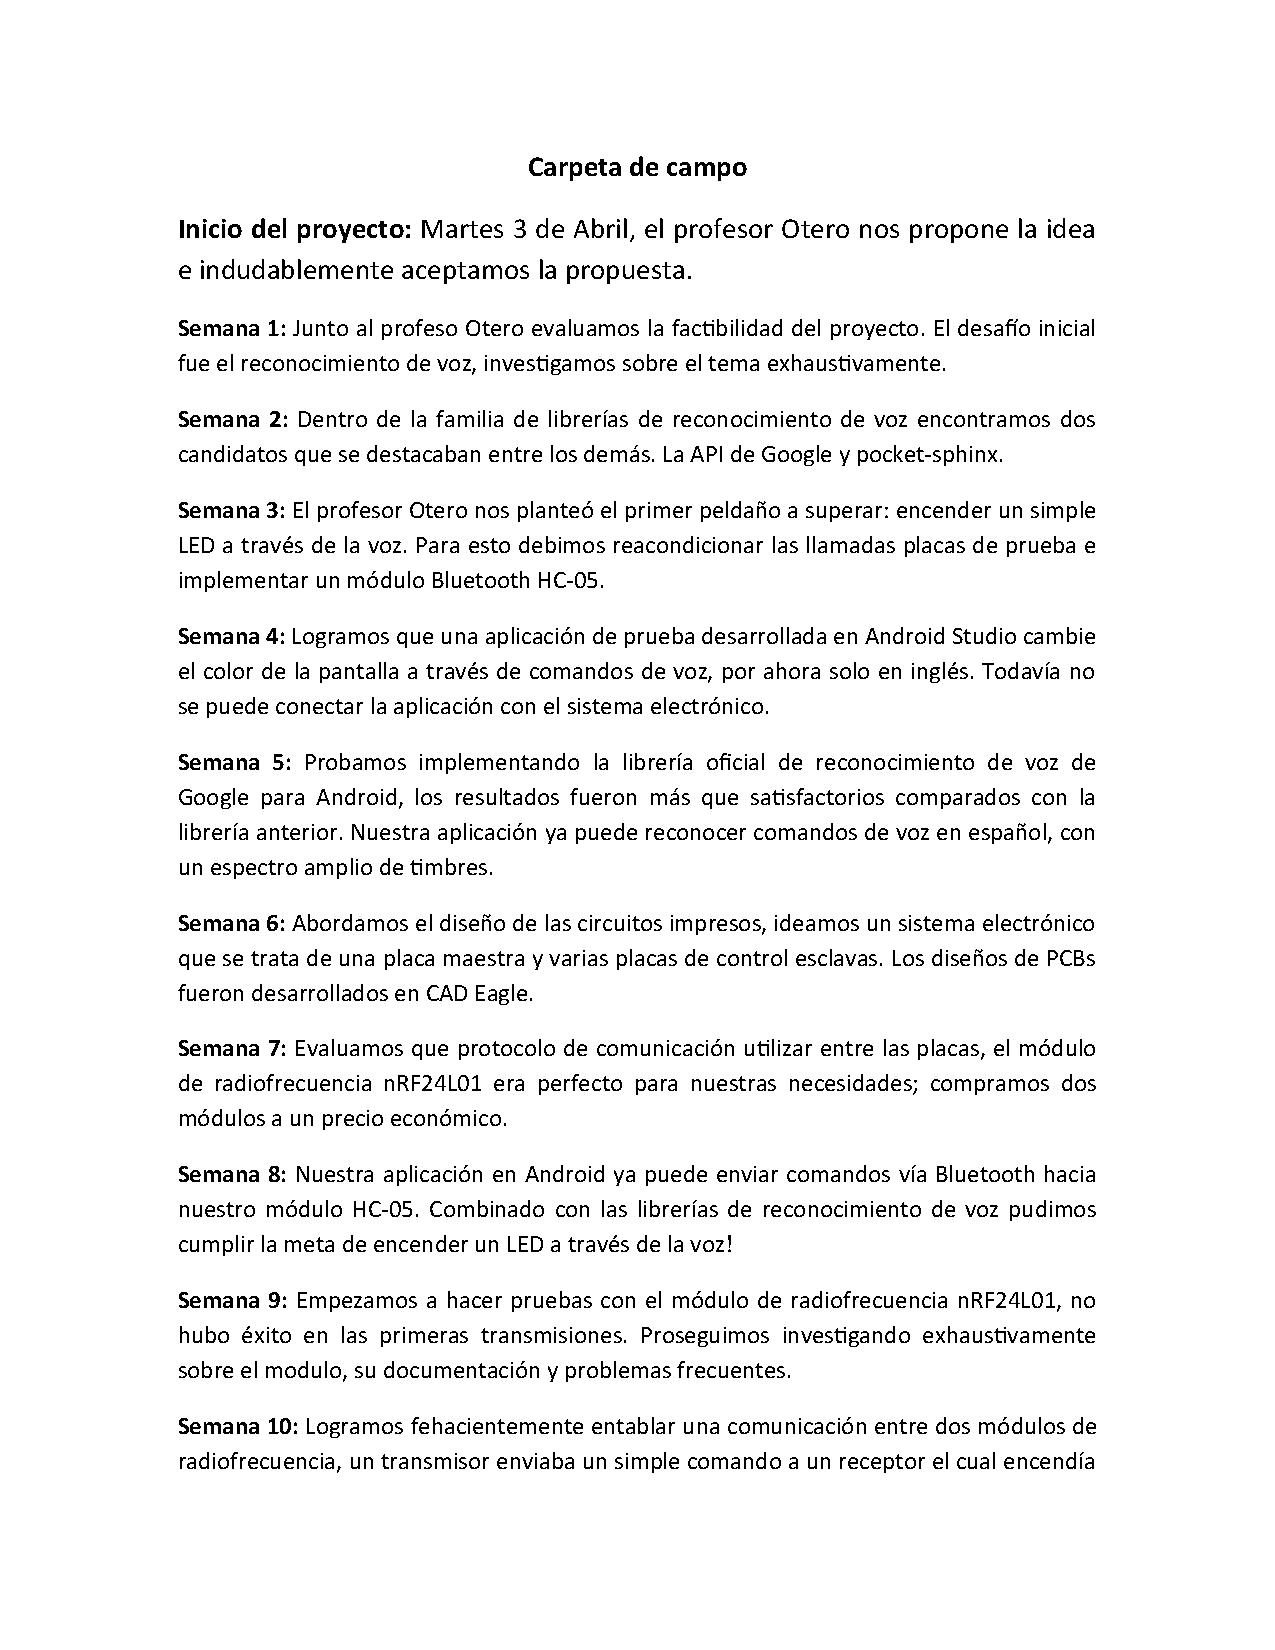
\includepdf[pages={1-},scale=1.00, pagecommand={}]{CARPETA_CAMPO.pdf}

\invisiblesection{ComposeCommand diagrama de flujo}
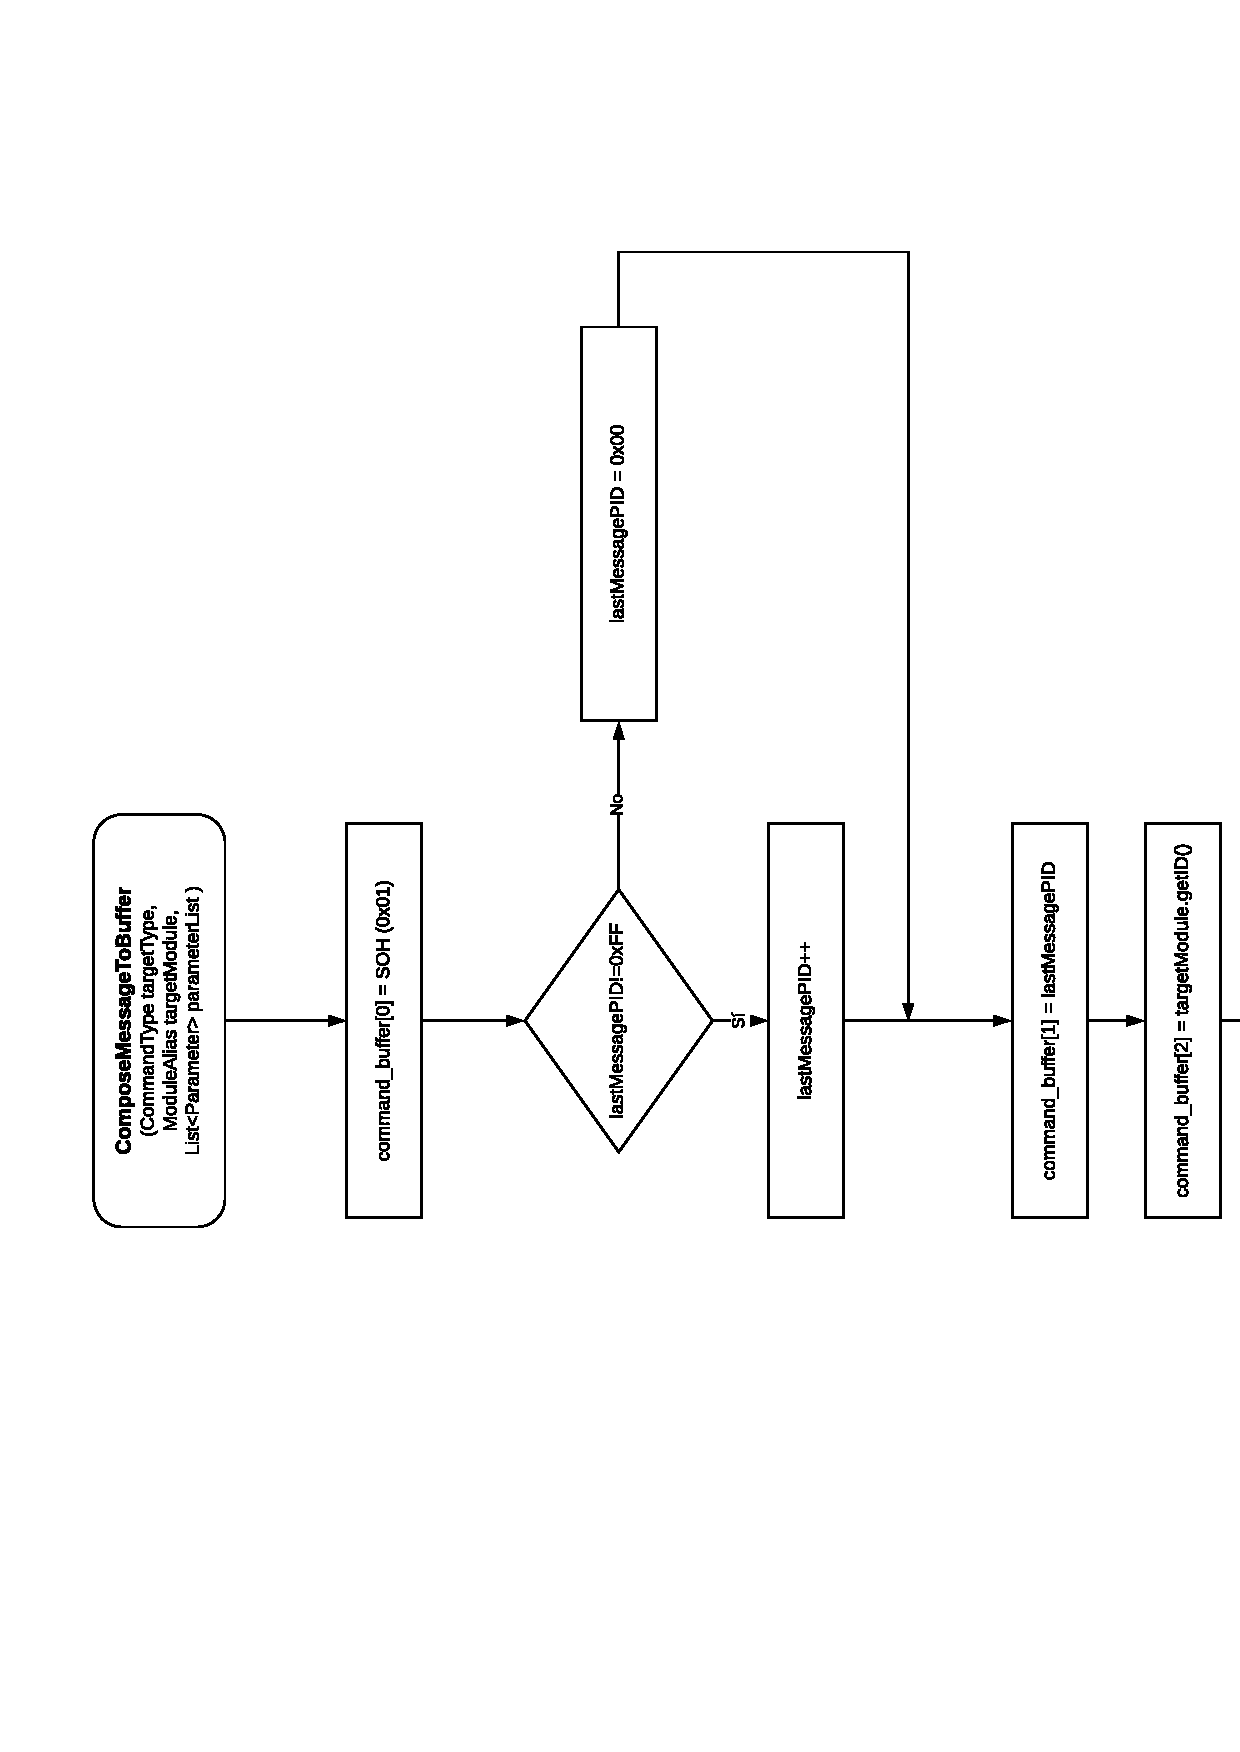
\includepdf[pages={1-},scale=1.00, pagecommand={}]{COMPOSE_FLOW_CHART.pdf}

\invisiblesection{DecomposeCommand diagrama de flujo}
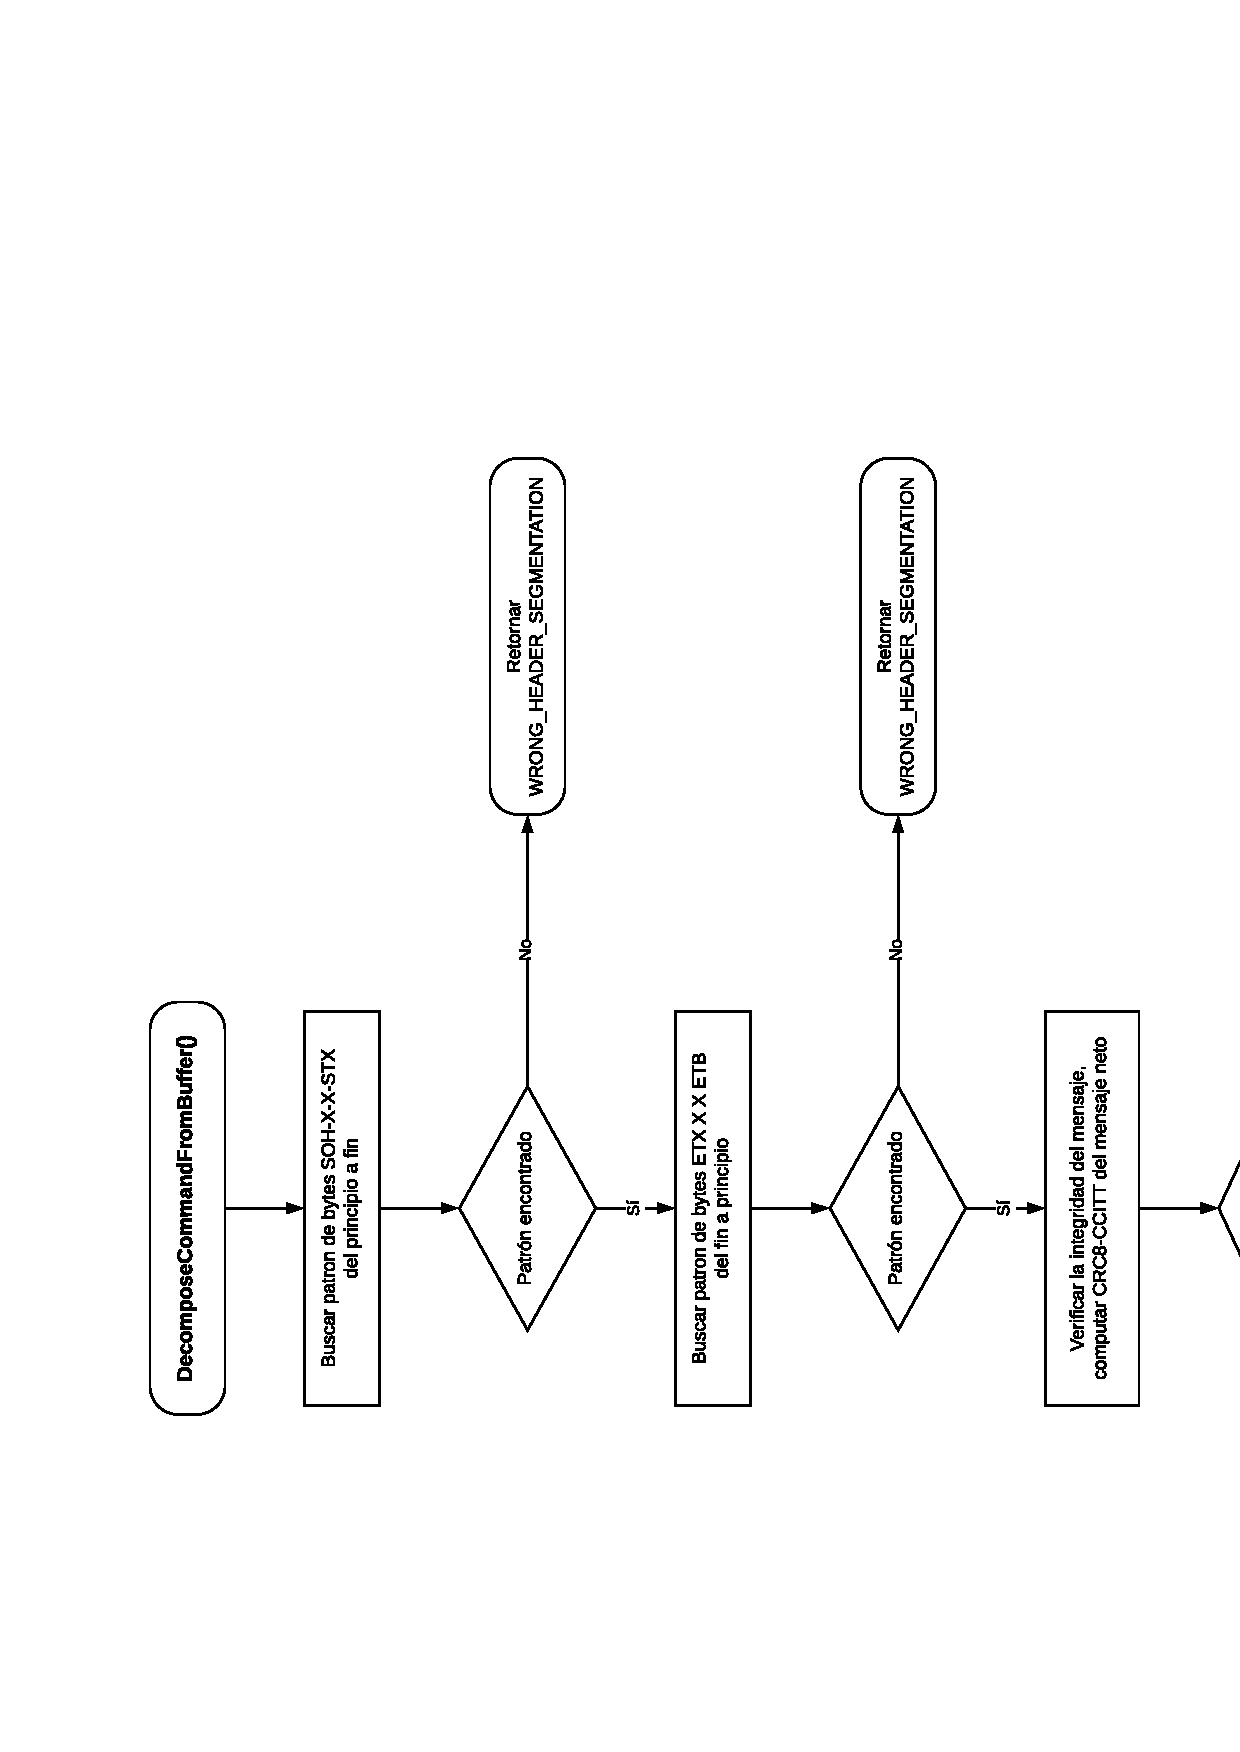
\includepdf[pages={1-},scale=1.00, pagecommand={}]{DECOMPOSE_FLOW_CHART.pdf}

\invisiblesection{Circuito impreso, módulo principal}
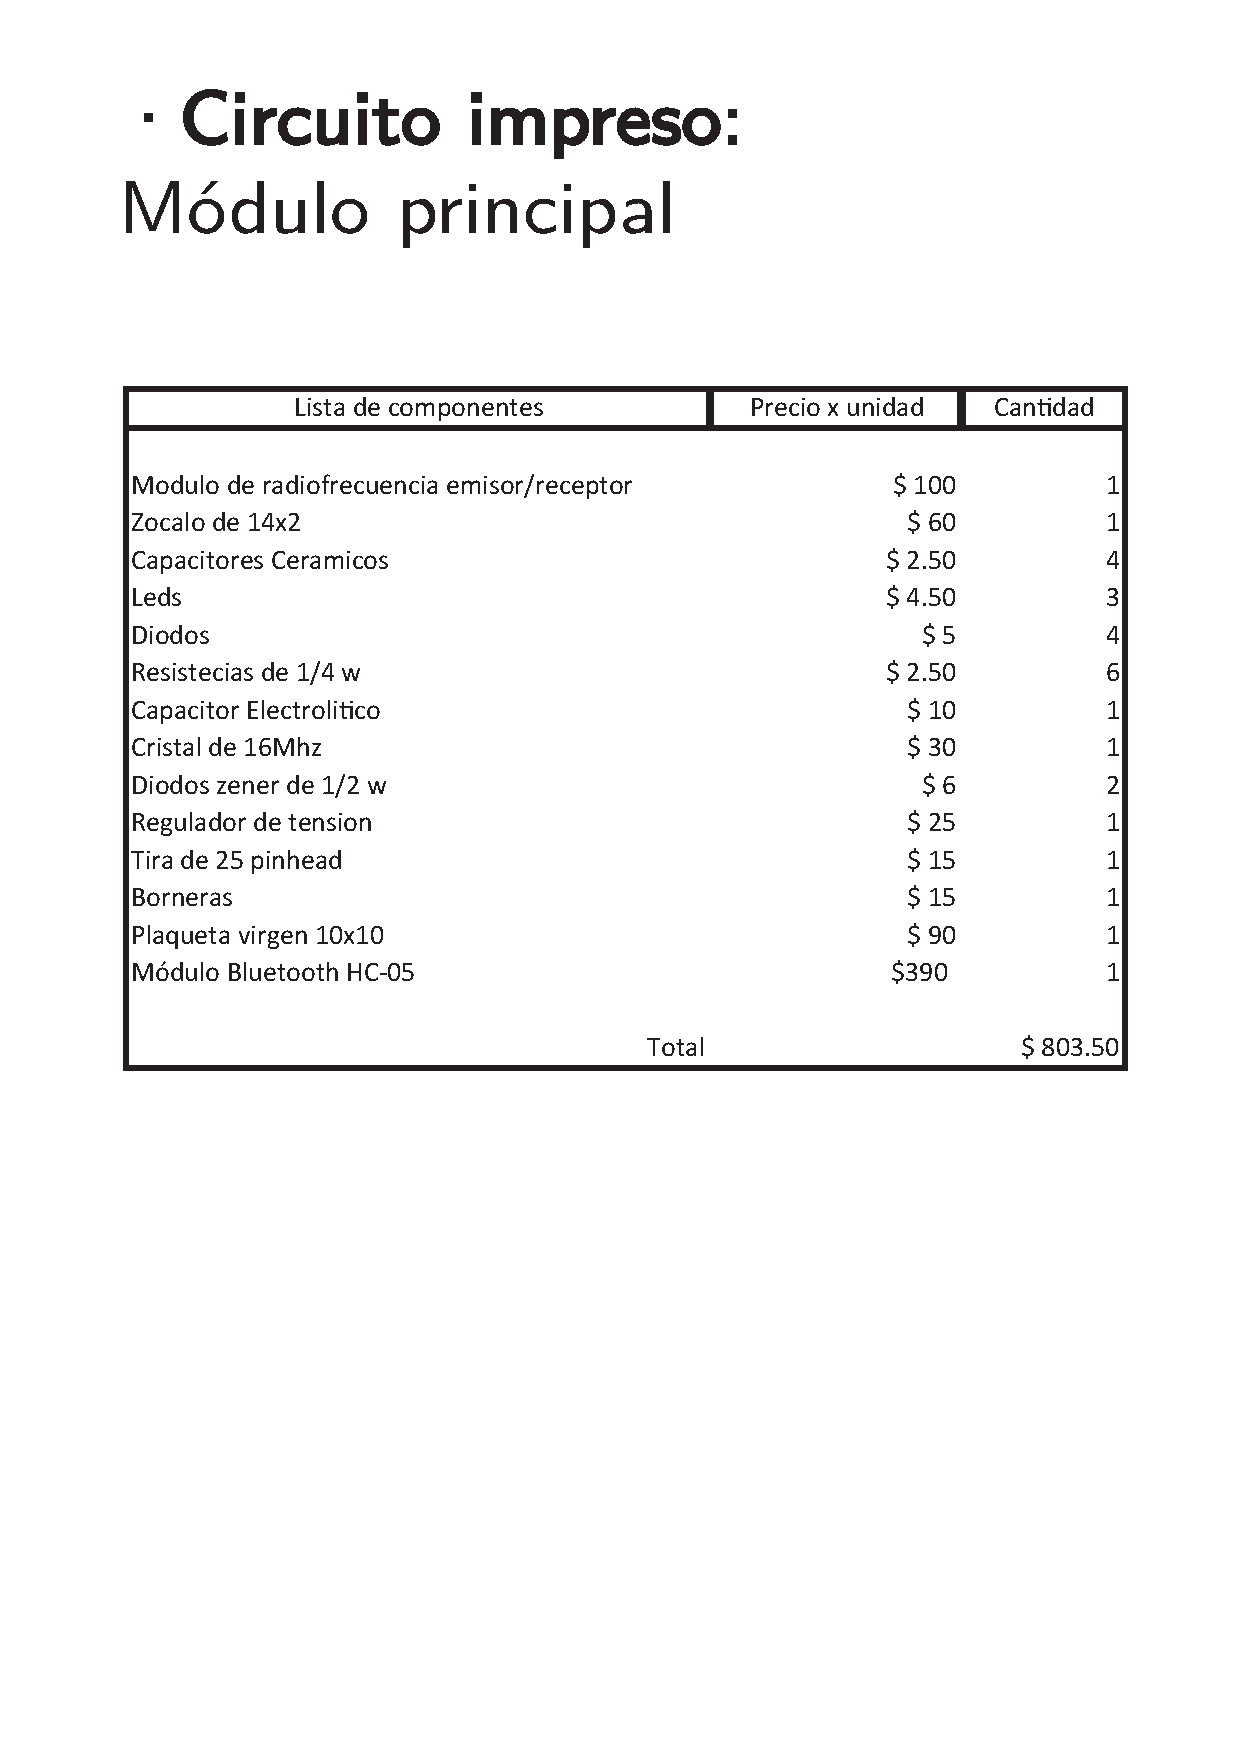
\includepdf[pages={1-},scale=1.00, pagecommand={}]{MAIN_PCB.pdf}

\invisiblesection{Circuito impreso, módulo de potencia}
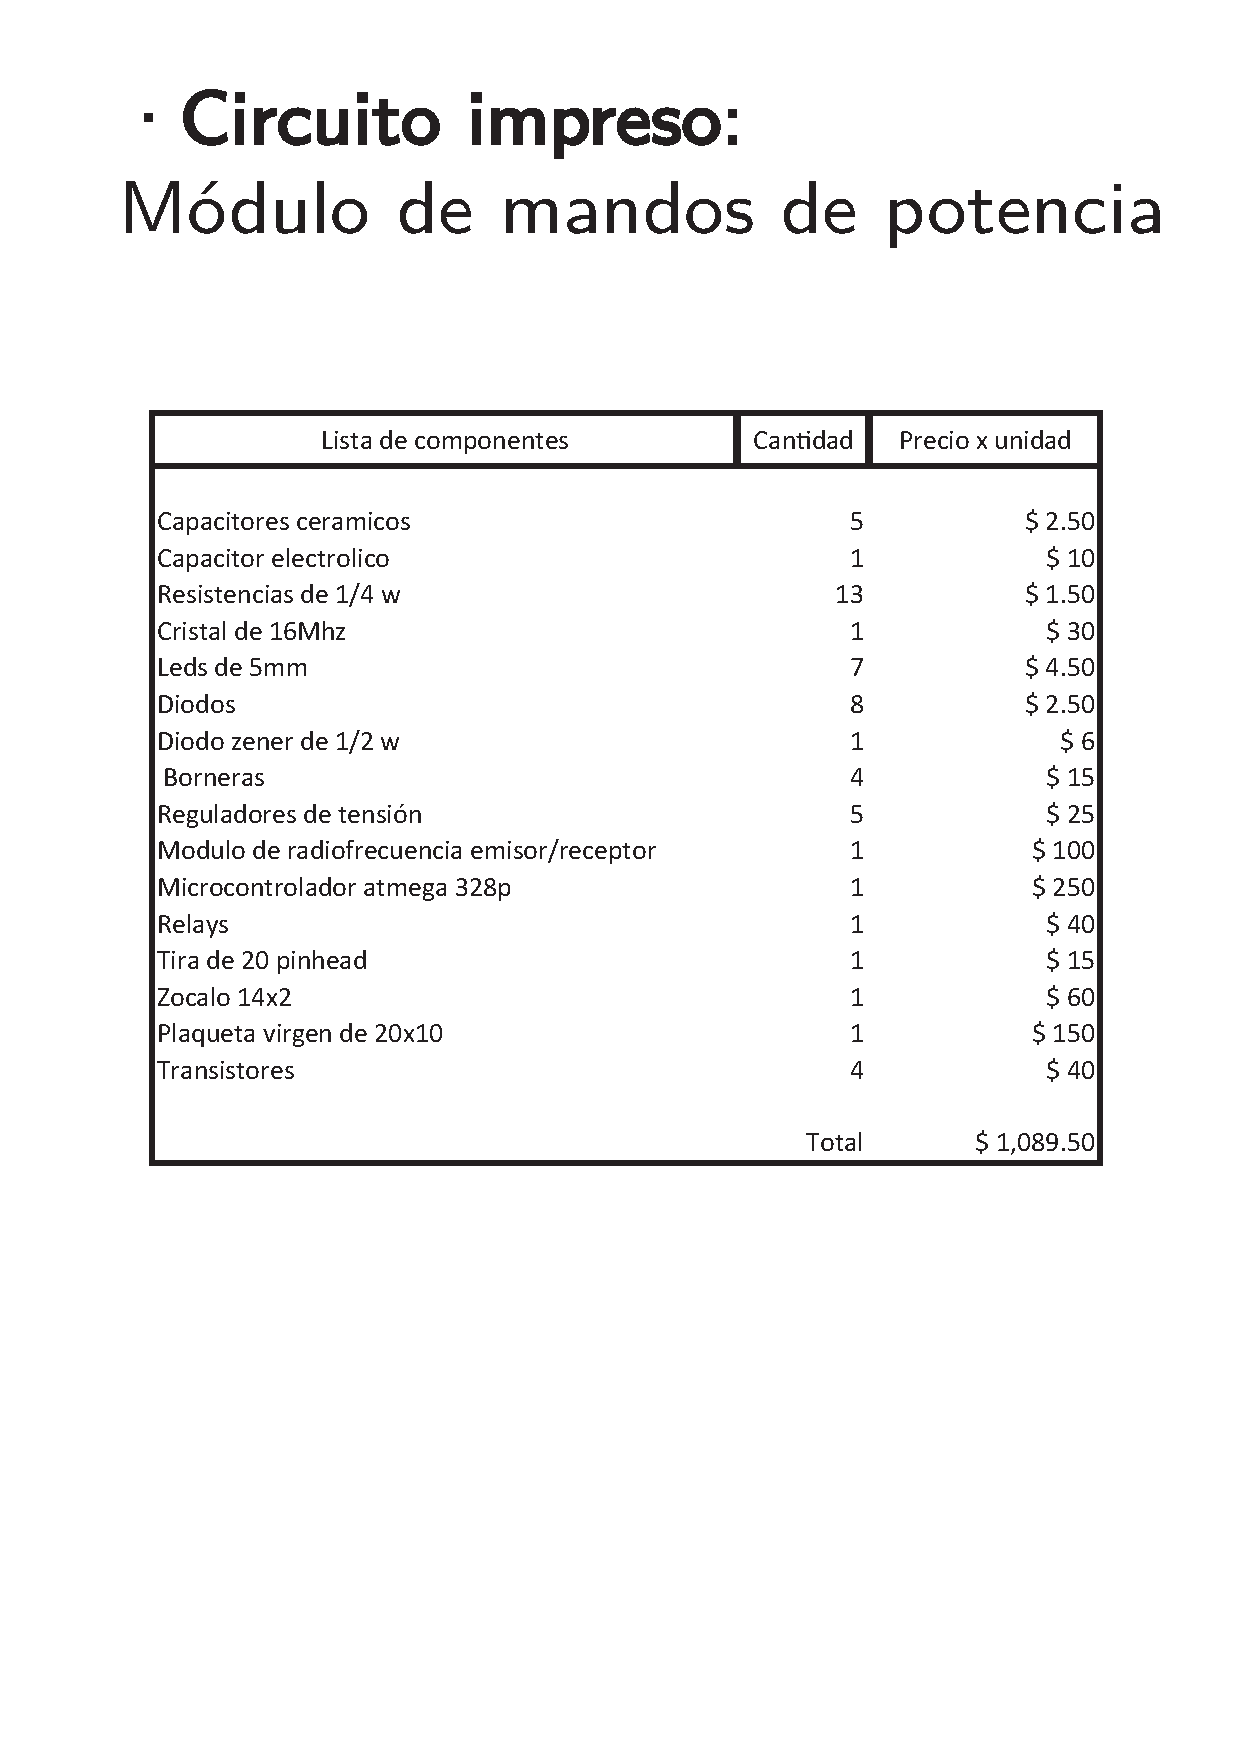
\includepdf[pages={1-},scale=1.00, pagecommand={}]{POWER_PCB.pdf}

\invisiblesection{Circuito impreso, módulo de mandos motrices}
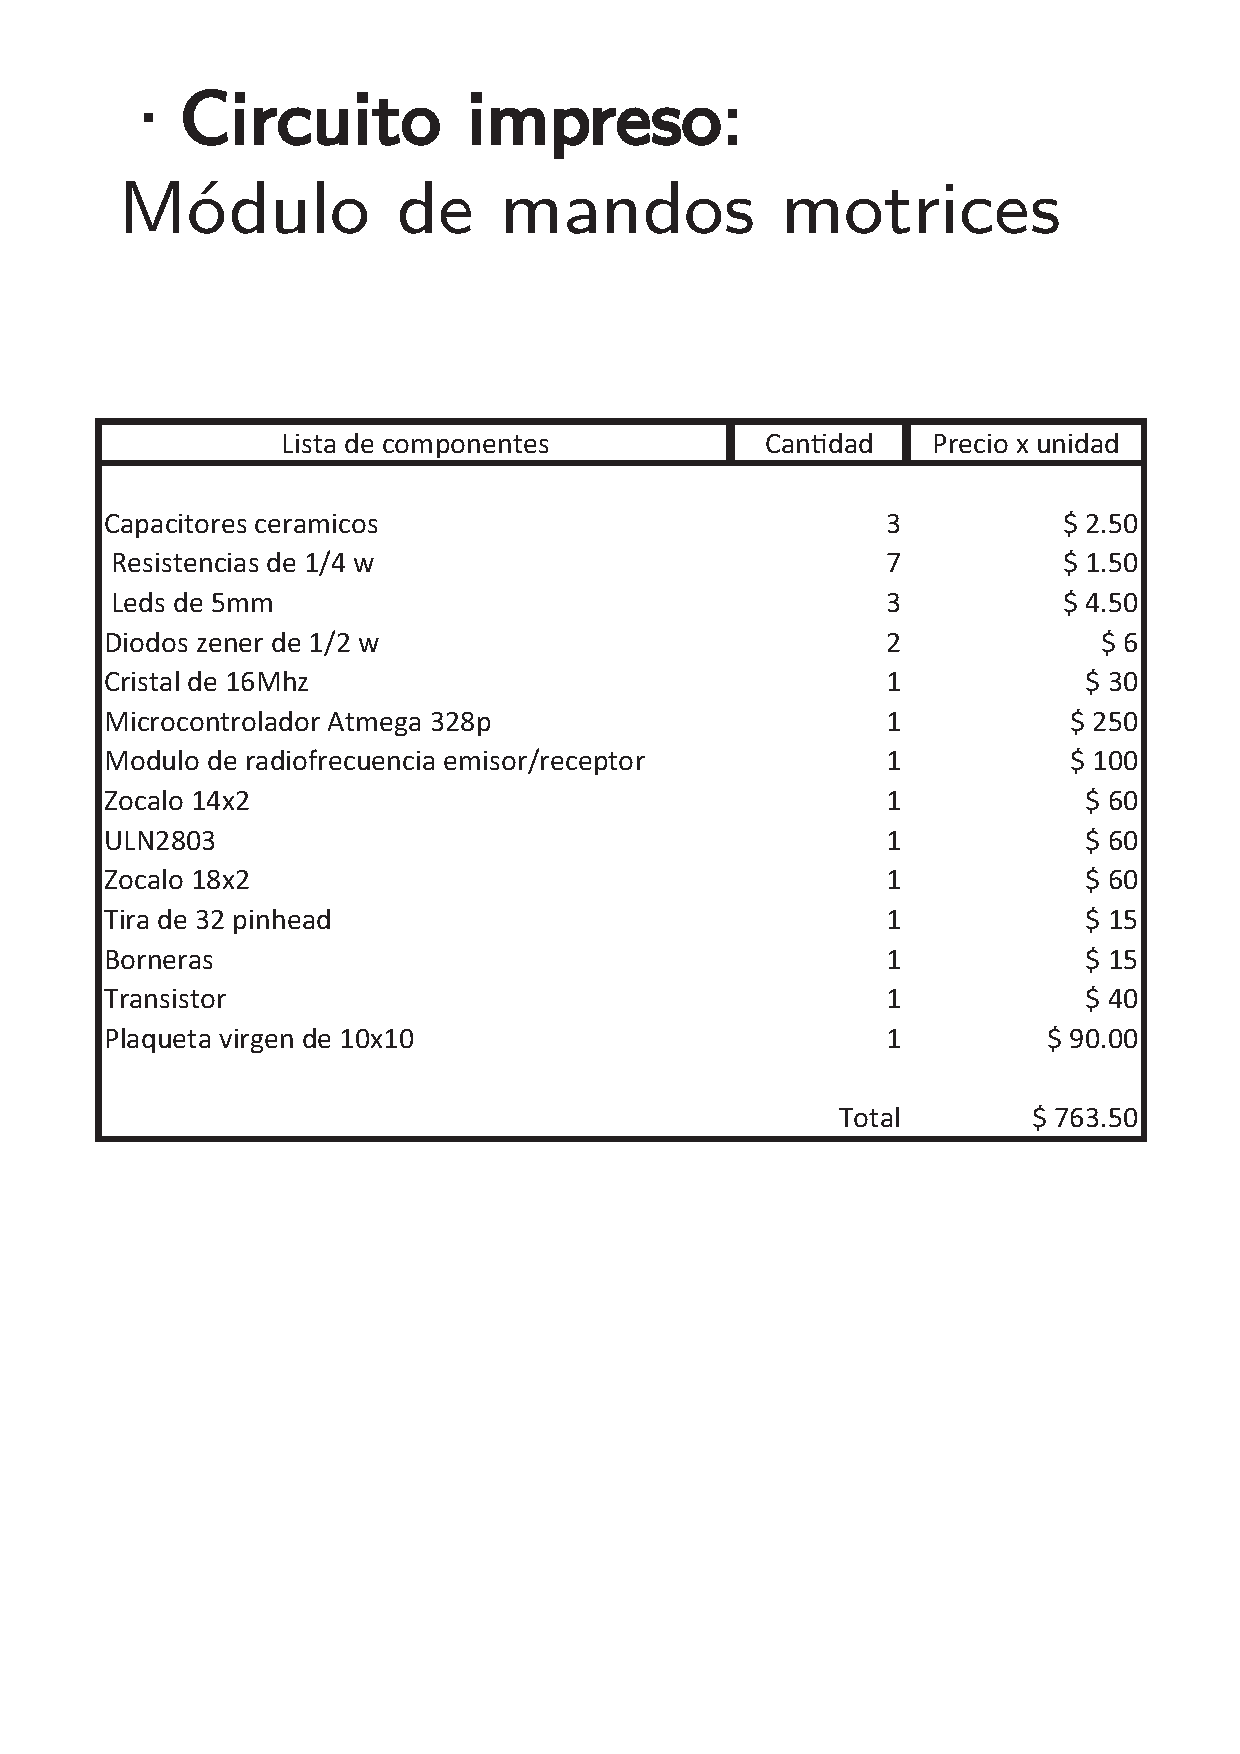
\includepdf[pages={1-},scale=1.00, pagecommand={}]{MOTOR_PCB.pdf}

\invisiblesection{Código de fuente, módulo principal}
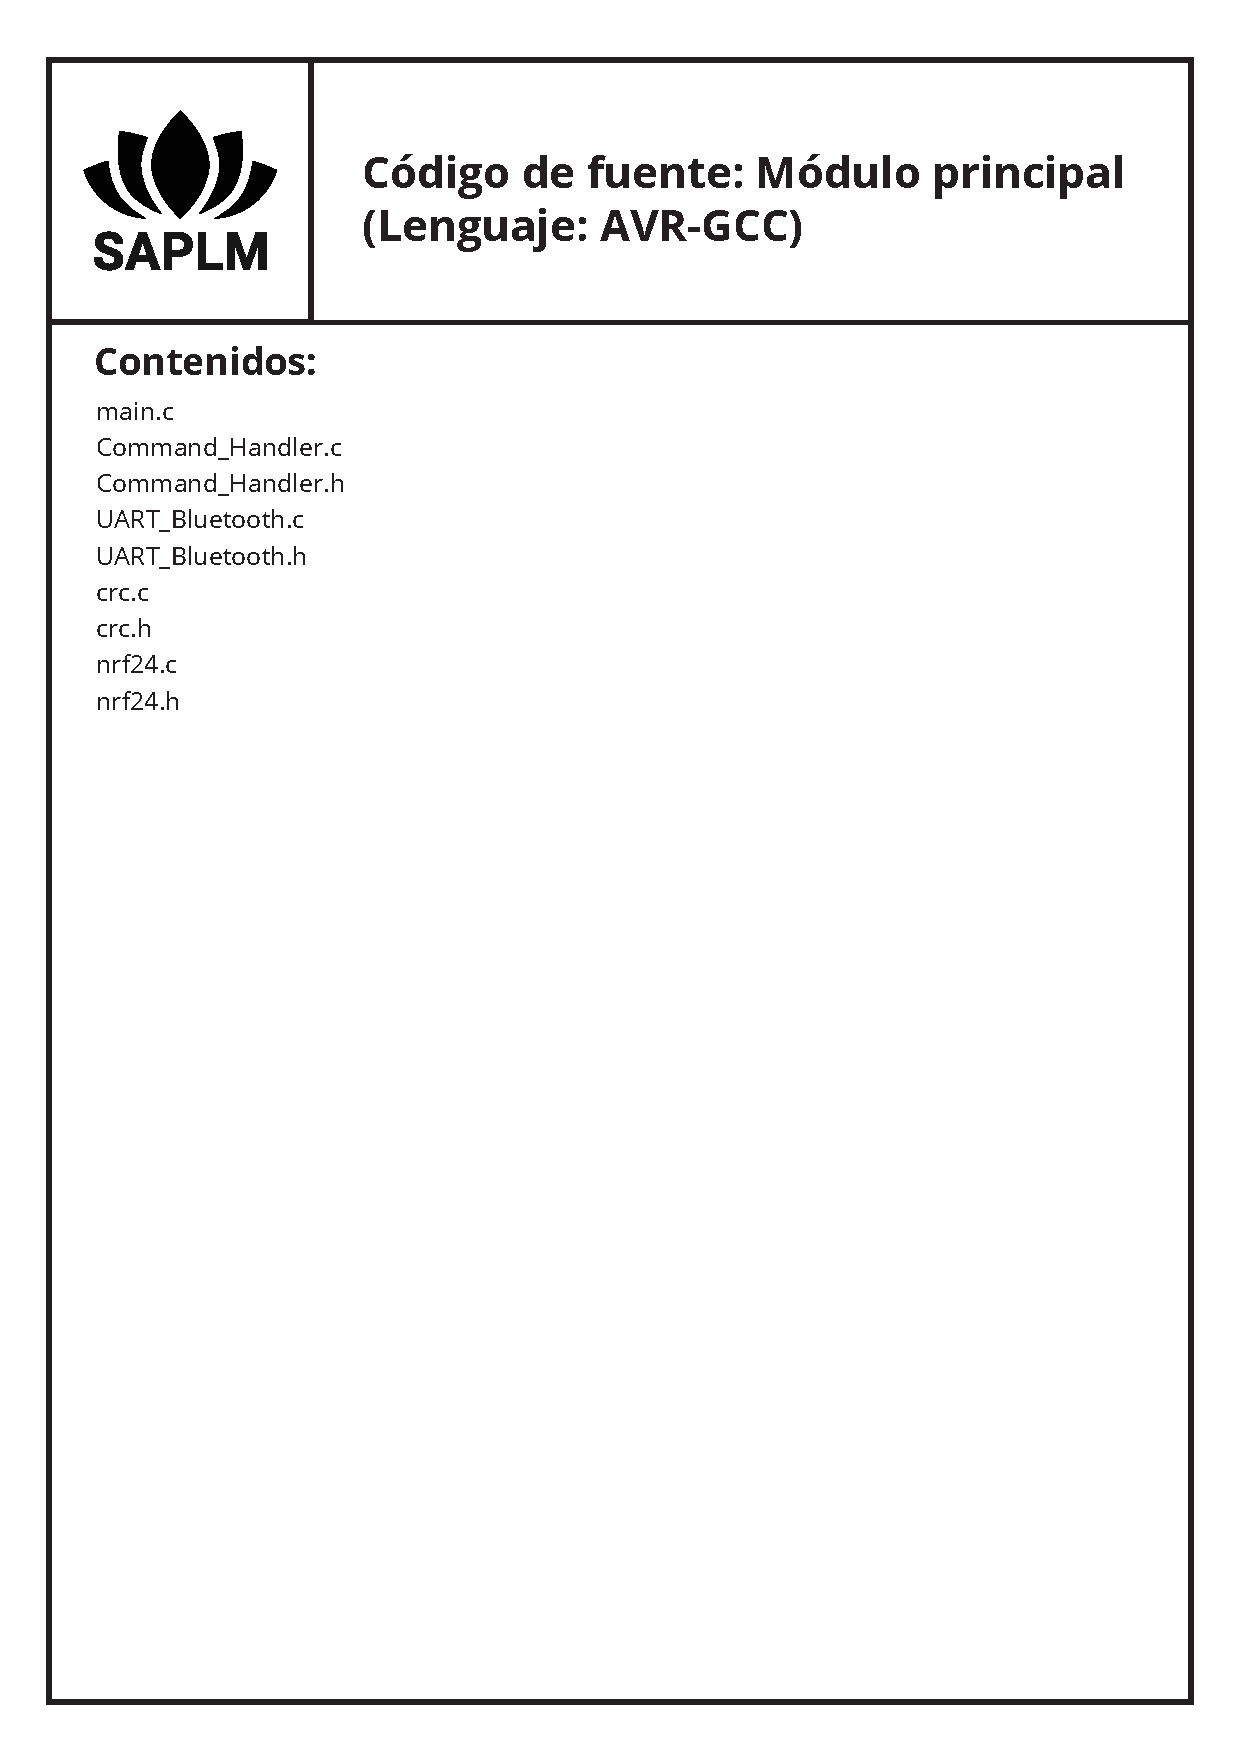
\includepdf[pages={1-},scale=1.00, pagecommand={}]{MAIN.pdf}

\invisiblesection{Código de fuente, módulo de potencia}
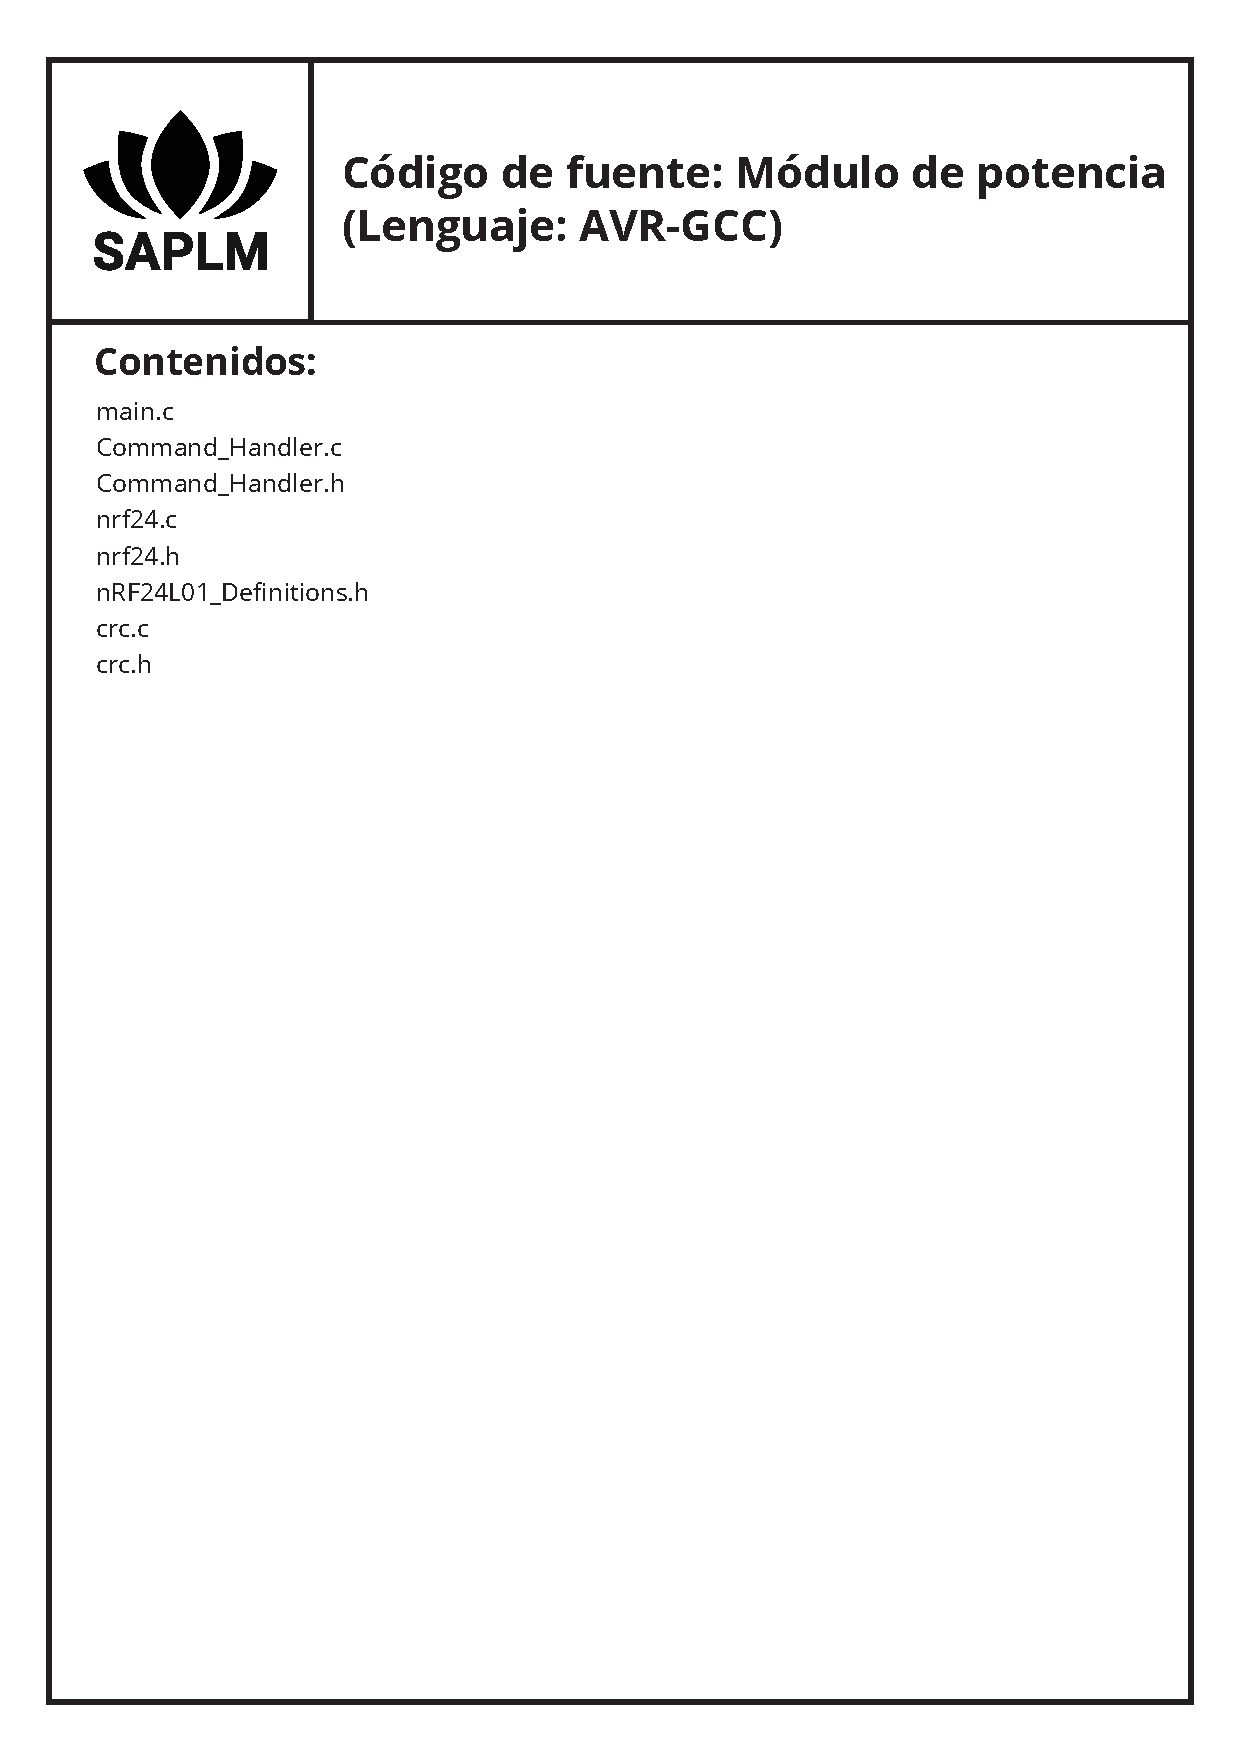
\includepdf[pages={1-},scale=1.00, pagecommand={}]{POWER2.pdf}

\invisiblesection{Código de fuente, módulo de mandos motrices}
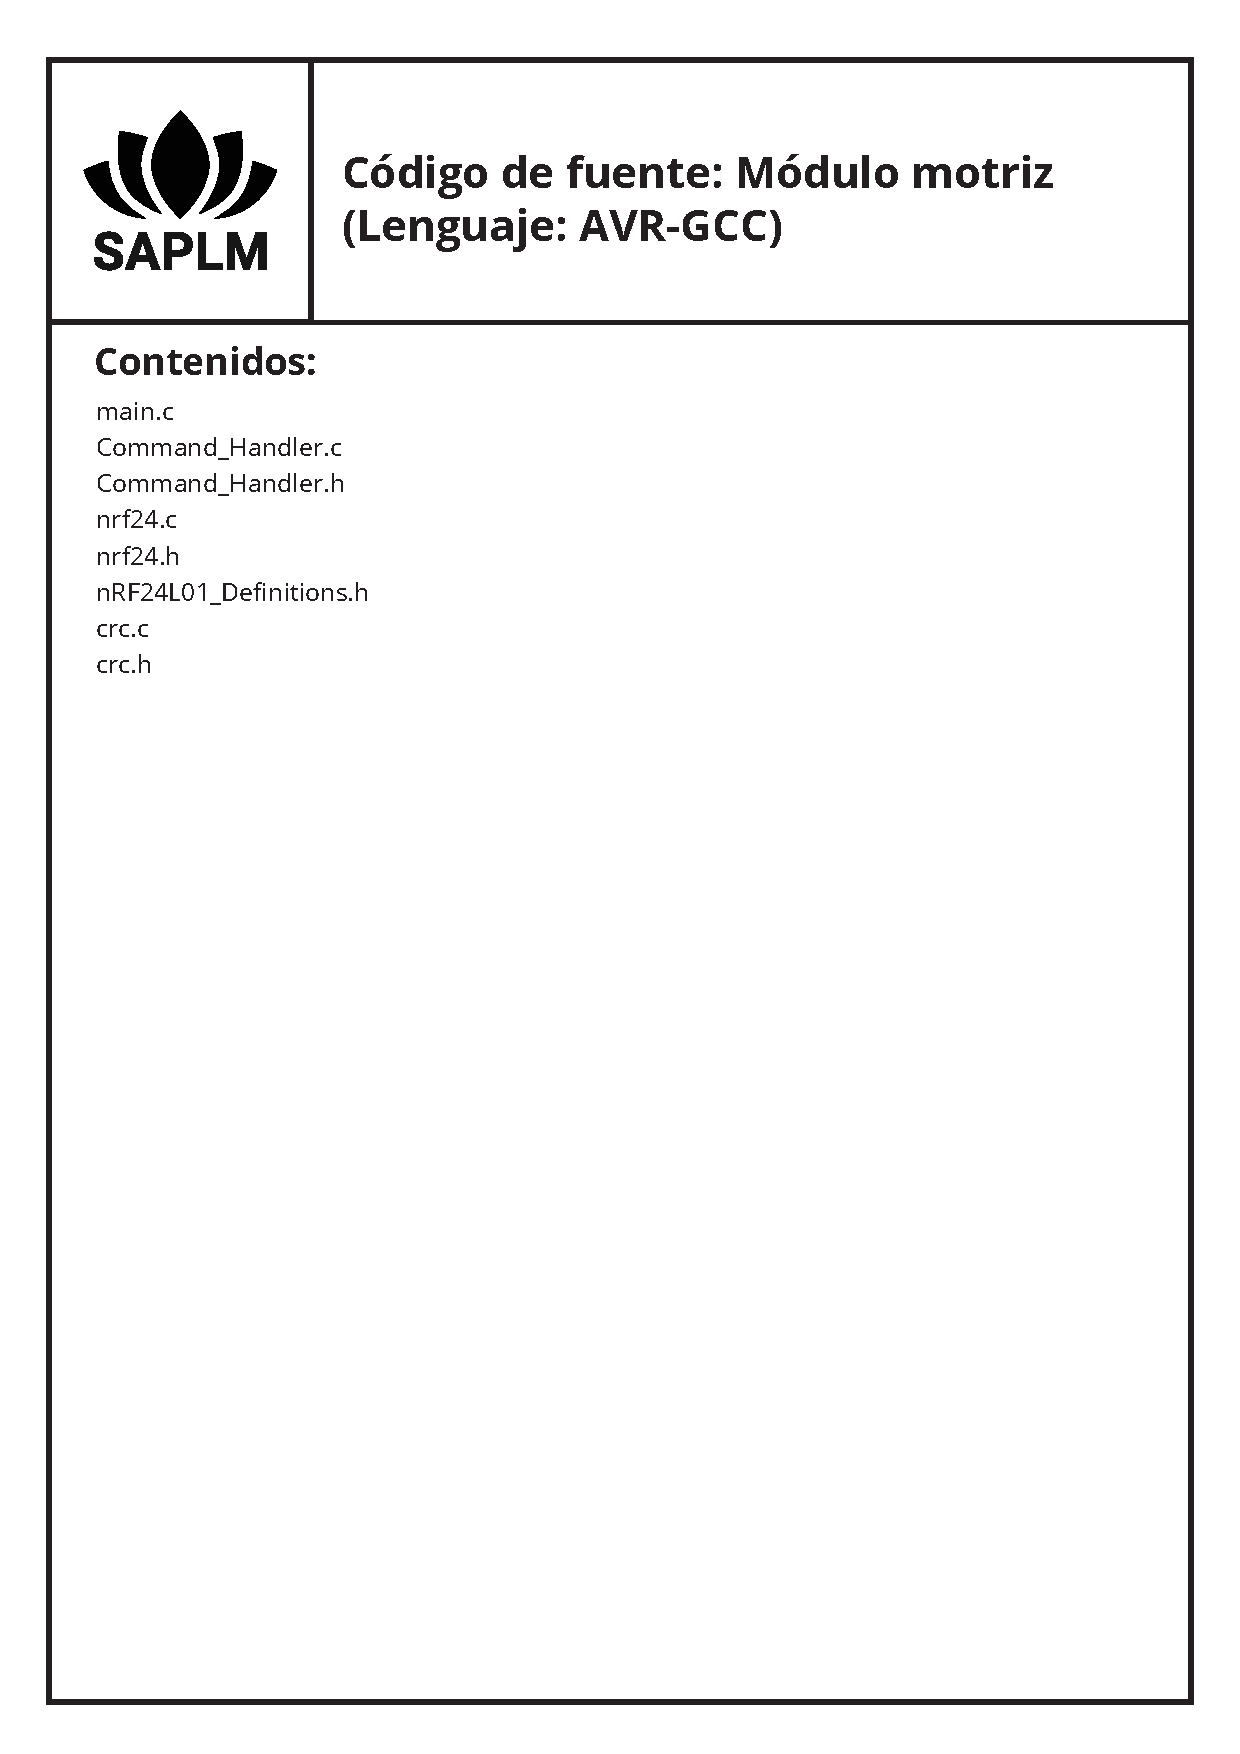
\includepdf[pages={1-},scale=1.00, pagecommand={}]{MOTOR.pdf}

\invisiblesection{Código de fuente, aplicación SAPLM}
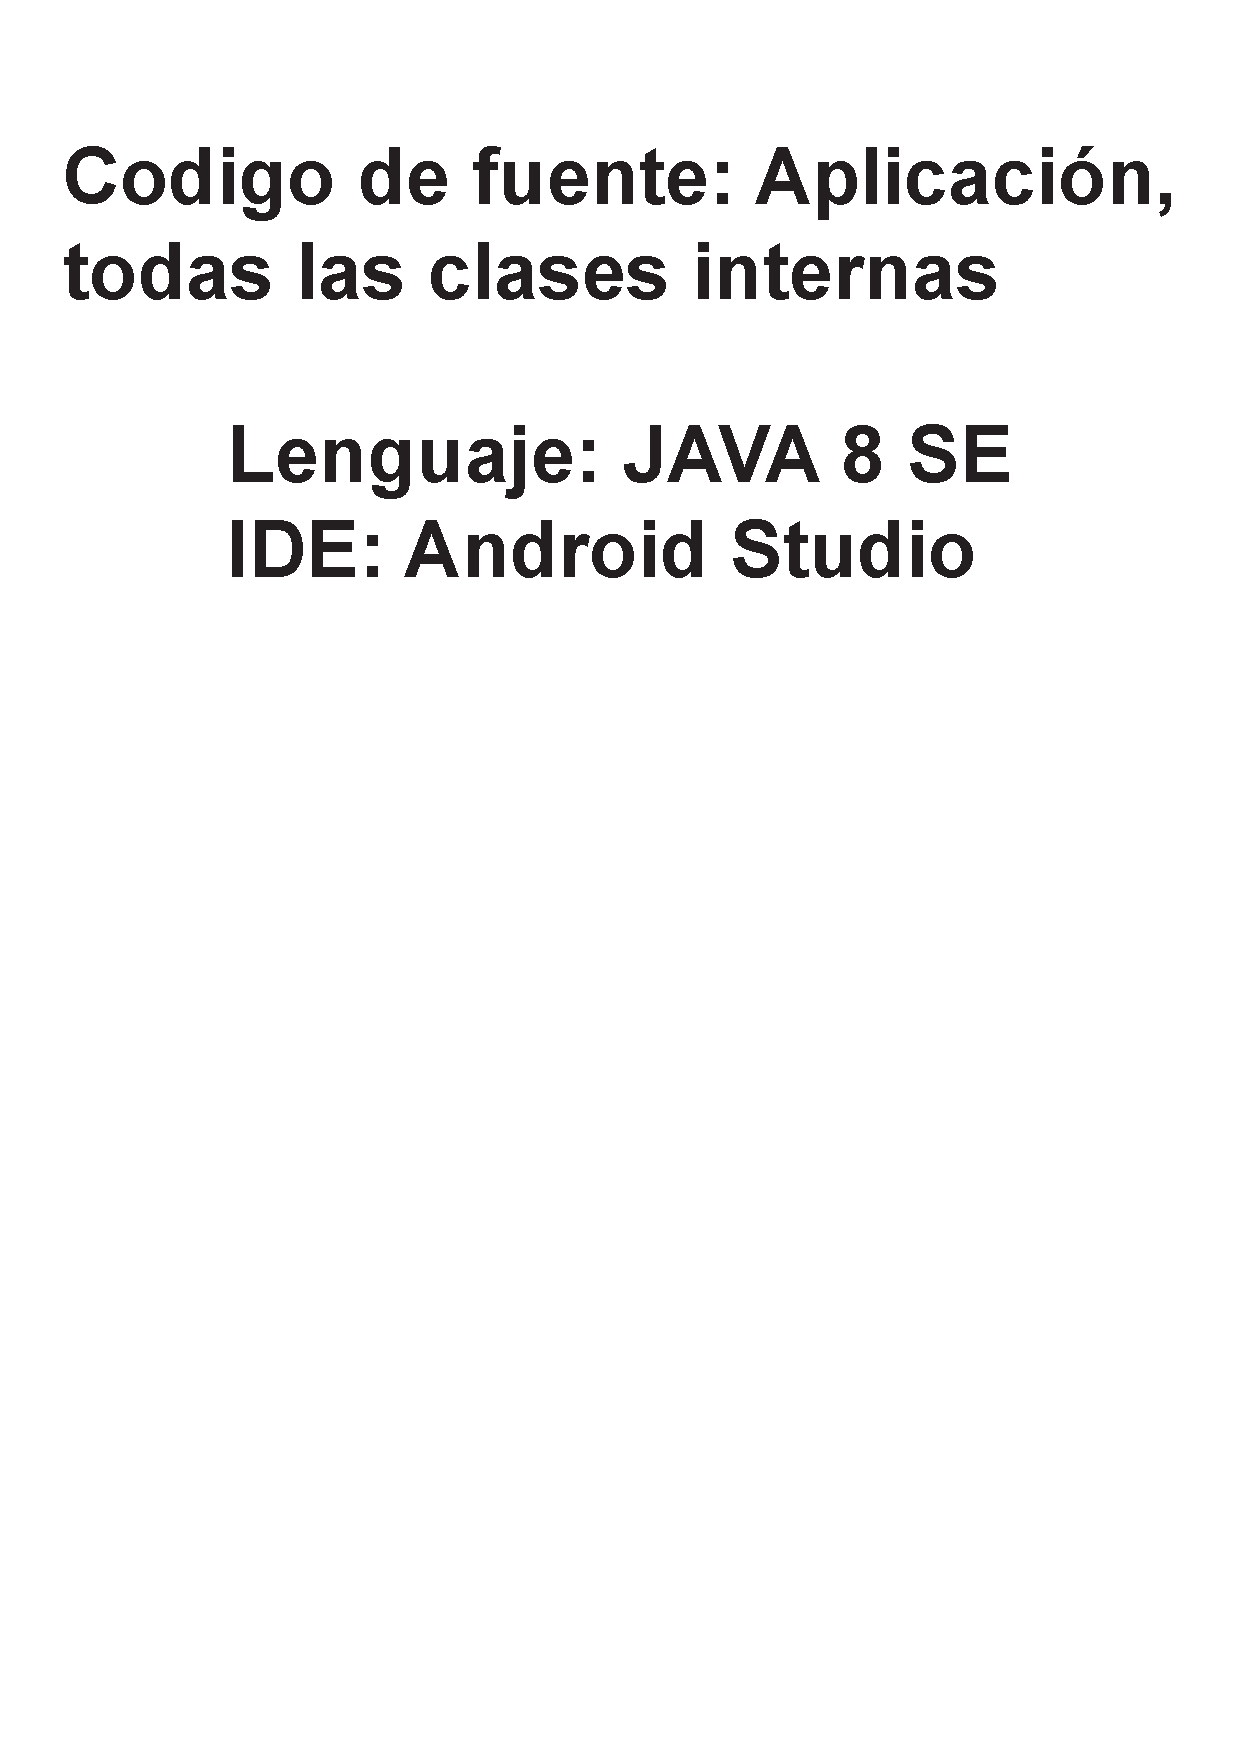
\includepdf[pages={1-},scale=1.00, pagecommand={}]{JAVA.pdf}

\invisiblesection{Código de fuente, Diseño de activities}
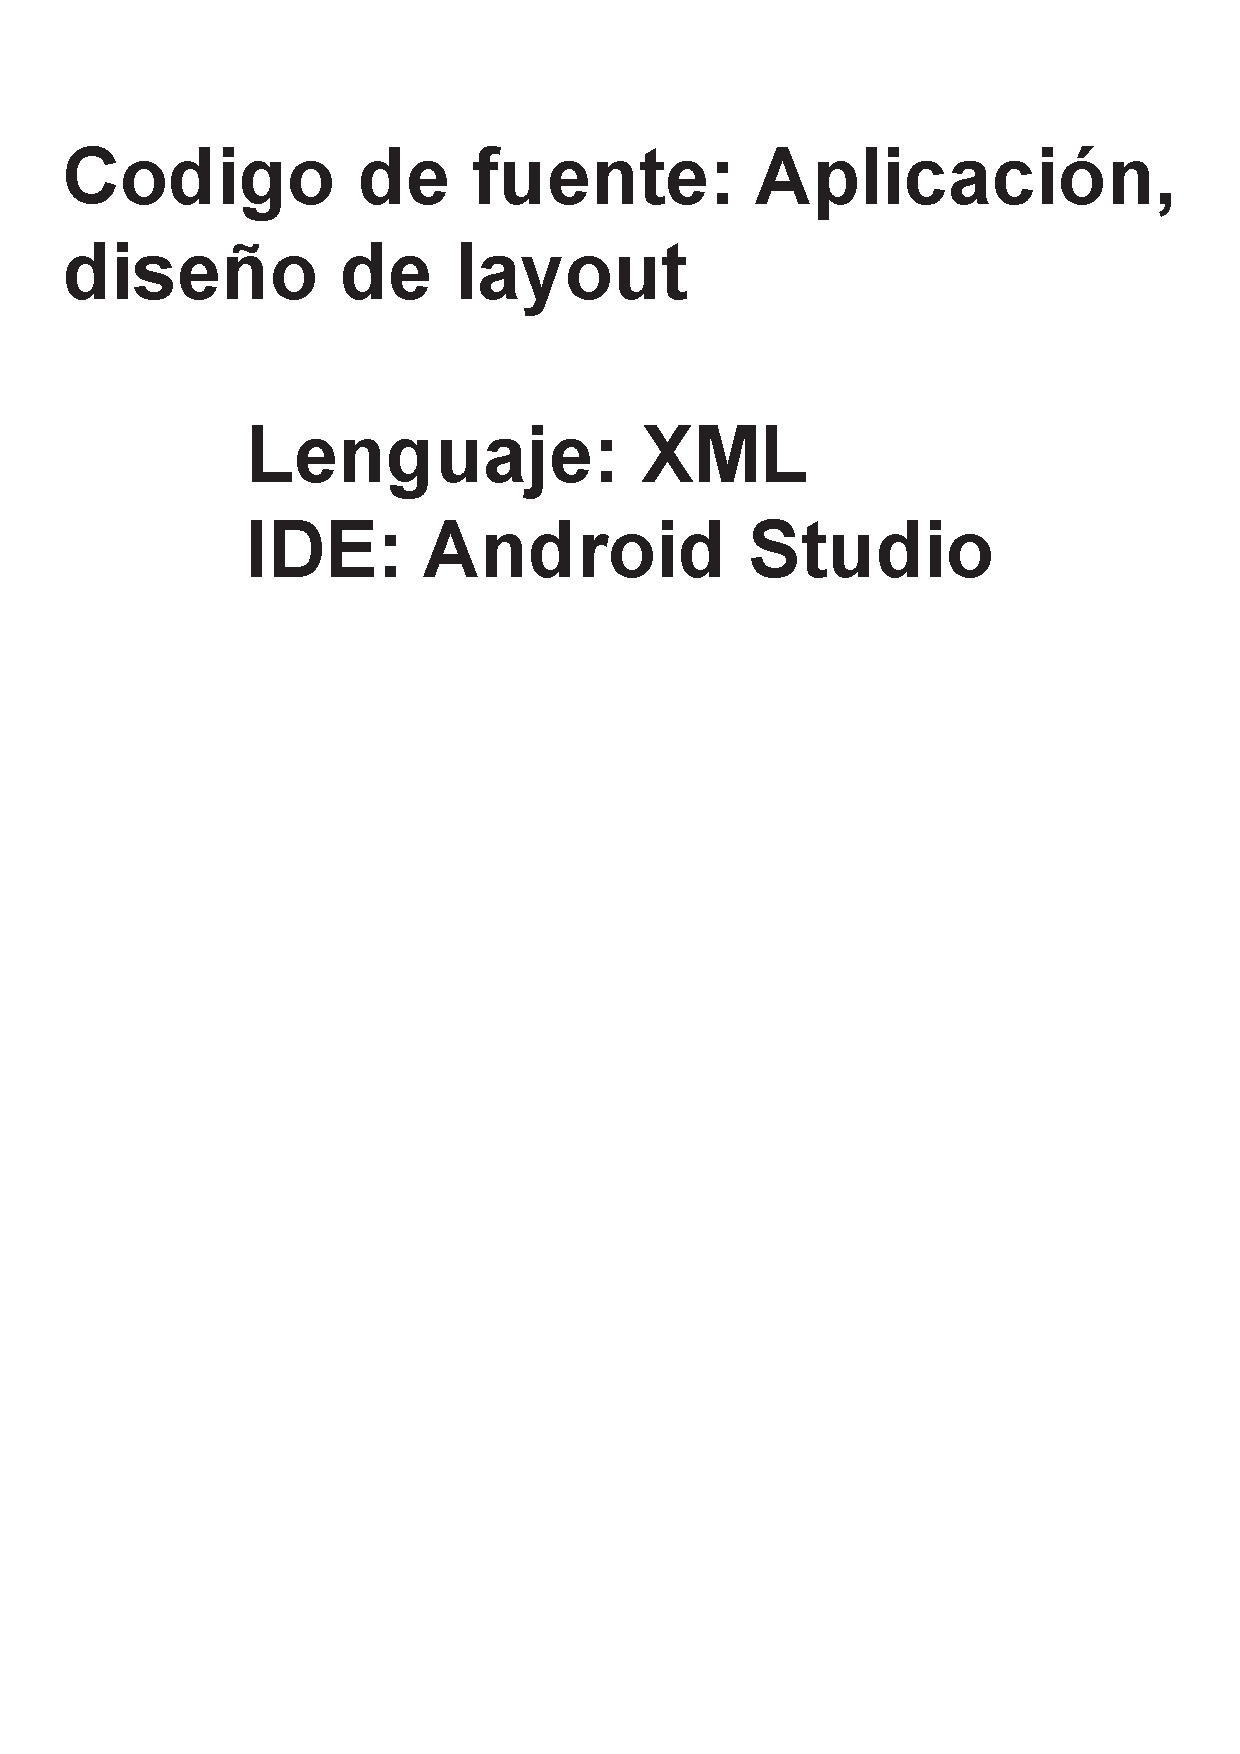
\includepdf[pages={1-},scale=1.00, pagecommand={}]{XML.pdf}

JAVA.pdf




\end{document}
